\chapter{DISTRIBUTED PASSIVE RFID COMPUTING}
\label{Section: Distributed Passive RFID Computing}
We study computing in a tag-based information system, and in particular, we consider its impact on continuous pervasive spaces. We use the word ``computing'' loosely. That is, we focus on several metrics in a distributed system that are related to computation ideas. In particular, as interrogators move through a continuous space with a dense tag deployment, the services they provide to users involve computations. We investigate these computation-motivated metrics on both a local and system level, in a simulation study.

\section{Local Computations}
\label{Section: Distributed Passive Computing: Local Computations}
Before providing the details of our simulation study, we first study computations at a local level. Because of tag multiplicity leading to the distributed nature of our tag deployments, these local computations have system-wide effects. So we first study the local effects. We provide simple expressions relating physical tag parameters to computing speed, in a small locality. In particular, assume computer instructions are stored in tags, with $r$ bits$/$instruction. Interrogators scan a set of tags, read the stored instructions, execute them, and then overwrite the storage with other instructions. For simplicity, we assume any data is stored as part of the instructions, so that we do not have to account for a separate storage category. Consider a physical space with tags. An interrogator is in the area, and scans $m$ tags. Each tag has $s$ bits of storage capacity. We assume singulation is linear in the number of tags, with a singulation rate of $\beta$ tags$/$s. (This may not be realistic in all situations. However, it suffices for us to generate a simple expression. Furthermore, many interrogator manufacturers provide a singulation rate, which we can easily apply to our expression.) The tag read throughput is $\gamma_{read}$ bits$/$s, and the tag write throughput is $\gamma_{write}$ bits$/$s. These correspond to the speeds at which the interrogator reads and writes data to a tag, respectively, once it knows its ID. We now have all the components to calculate the number of instructions executed (by the interrogator) per unit time. The number of instructions executed in one session (scan, read, execute, and write) is $\frac{s}{r}m$. The time of one session consists of the scan time, the read time, and the write time. We assume that the execution time is negligible, since the other times are bits transmitting over the wireless medium, which dominates local calculations. The scan time is $\frac{1}{\beta} m$. The read and write times are $\frac{s}{\gamma_{read}}m$ and $\frac{s}{\gamma_{write}}m$, respectively. Therefore, the computing speed, $\sigma$, in number of instructions$/$s is the following:
\begin{eqnarray}
\sigma = \frac{\frac{s}{r}m}{\frac{1}{\beta} m + \frac{s}{\gamma_{read}}m + \frac{s}{\gamma_{write}}m } =  \frac{\frac{1}{r}}{\frac{1}{s}\frac{1}{\beta} + \frac{1}{\gamma_{read}} + \frac{1}{\gamma_{write}} }.
\label{Equation: Computing Speed 1}
\end{eqnarray}
The second part of Equation (\ref{Equation: Computing Speed 1}) is very intuitive, and can actually be derived directly from a unit analysis. That is, $\frac{1}{r}$ represents how many instructions can be represented in one bit of storage. (Obviously we need more than one bit of storage$/$instruction. But this is a unit analysis.) As well, $\frac{1}{\beta}$ is the scan time$/$tag and $\frac{1}{s}$ is the number of tags$/$bit of storage. Thus, $\frac{1}{s}\frac{1}{\beta}$ is the scan time$/$bit; $\frac{1}{\gamma_{read}}$ and $\frac{1}{\gamma_{write}}$ are the read and write times$/$bit, respectively. Therefore, Equation (\ref{Equation: Computing Speed 1}) is interpreted as follows:
\begin{eqnarray}
\sigma &= &\mbox{number of instructions$/$s}  \nonumber \\
& = &\frac{\mbox{number of instructions$/$bit}}{\mbox{scan time$/$bit} + \mbox{read time$/$bit} + \mbox{write time$/$bit} }.
\label{Equation: Computing Speed 2}
\end{eqnarray}
The number of tags, $m$, that is scanned by the interrogator is not part of the expression. Even the tag storage size, $s$, is not part of the expression. These are naturally abstracted out, since computing speed is a only a function of how fast the interrogator can transmit data from and to tags. The units representing data quantities are normalized away. (Interrogator scan range is not in the expression because it affects the number of scanned tags, which is a data quantity.) Of course, this is true only when we assume a fixed singulation rate and fixed data rates. Practically, within a controlled range of interrogator scan powers, these rates may not vary much. Therefore, even though within this scan power range the interrogator may be able to capture different numbers of tags, the computing speed is still fairly constant. As a system administrator, thus changing the tag density (through increases or decreases in tag deployment rate) may not significantly change the performance of applications that rely on computing in small localities.

Consider instruction sets with $r \in \{32, 64\}$ bits$/$instruction. Commodity passive tags typically have $s = 512$ bits of storage. The singulation rates of modern interrogators are usually rated at over $\beta = 100$ tags$/$s, and can be as high as $\beta = 1000$ tags$/$s. Gen 2 UHF EPC technology has tag read and tag write times of $640$ kbps and $128$ kbps, respectively \cite{2005 Fischer}. Using Equation (\ref{Equation: Computing Speed 1}), we see the range of computing speeds (in instructions$/$s) in Table \ref{Table: Range of computing speeds (instructions/second).}.

Now we provide simple expressions showing energy consumption. Assume the interrogator has scan power $P$ associated with scan range $R$. Then, $P = \alpha R^{\delta}$, where $\alpha > 0$ is a proportionality constant, and $\delta \geq 2$ is the path loss exponent. Assume the spatial tag density is $\rho$. Therefore, the singulation time (not the entire computation time) is $\frac{\rho \pi R^2}{\beta}$. So the energy consumed in one singulation session is $\frac{\rho \pi R^2}{\beta} \alpha R^{\delta} = \frac{\alpha \rho \pi R^{2 + \delta}}{\beta}$. Note that the energy consumed per tag scanned is $\frac{\alpha R^{\delta}}{\beta}$. That is, as we increase the interrogator power, we can scan more tags. However, the unit energy consumed increases.


\section{System Model}
\label{Section: Distributed Passive RFID Computing: System Model}
Our physical space is a disk of radius $r$ with $n$ tags randomly located on it, according to a uniform distribution. At any given moment, there is only one interrogator in the disk. Interrogators each have a circular scan range of $R_I$. The interrogator dynamics are as follows:
\begin{enumerate}
\item The interrogator chooses a random starting location in the disk, according to a uniform distribution.
\item The interrogator scans all the tags in its range (and records their IDs).
\item The interrogator does the following for $m$ times:
\begin{enumerate}
\item The interrogator moves to another random location in the disk (according to a truncated L\'{e}vy distribution, which we detail later). 
\item The interrogator scans all the tags in its range (and records their IDs). 
\item The interrogator stays at this location for a random period of time (according to another truncated L\'{e}vy distribution, which we detail later). 
\end{enumerate}
\item The interrogator leaves the disk.
\end{enumerate}
These steps are repeated by a total of $N$ interrogators one after another. That is, an interrogator starts at a random location, moves $m$ times, and then leaves the system. Afterward, another interrogator appears, and performs the same steps, up to the $N^{th}$ interrogator. All probability distributions described above are mutually independent of each other, and generated samples within the same distribution themselves are independent across time.

Our system uses multiple truncated L\'{e}vy distributions. We outline the L\'{e}vy and truncated L\'{e}vy distributions. A L\'{e}vy random variable $L$ has the probability distribution function $f_L\left(l\right)$ and the cumulative distribution function $F_L\left(l\right)$ as follows:
\begin{eqnarray}
f_L\left(l\right) = \sqrt{\frac{\alpha}{2\pi}} \frac{e^{-\alpha/2l}}{l^{3/2}}, l \geq 0, \mbox{ and}
\label{Equation: Levy PDF}
\end{eqnarray}
\begin{eqnarray}	
F_L\left(l\right) = \mbox{erfc}\left(\sqrt{\frac{\alpha}{2l}}\right), l \geq 0,
\label{Equation: Levy CDF}
\end{eqnarray}
where $\alpha > 0$ is a scale parameter and $\mbox{erfc}\left(x\right) = \frac{2}{\sqrt{\pi}} \int_x^{\infty}e^{-t^2}dt$ is the complementary error function. A truncated L\'{e}vy random variable is a L\'{e}vy random variable where all the probability mass after a given maximum value $l^{(max)} > 0$ is zeroed out, and the rest of the probability mass is rescaled accordingly. That is, a truncated L\'{e}vy random variable, $L_T$, has the following distribution functions:
\begin{eqnarray}
f_{L_T}\left(l\right) = \frac{f_L\left(l\right)}{F_L\left(l^{(max)}\right)}, 0 \leq l \leq l^{(max)}, \mbox{ and}
\label{Equation: Truncated Levy PDF}
\end{eqnarray}
\begin{eqnarray}
F_{L_T}\left(l\right) = \frac{F_L\left(l\right)}{F_L\left(l^{(max)}\right)}, 0 \leq l \leq l^{(max)}
\label{Equation: Truncated Levy CDF}
\end{eqnarray}

In the interrogator dynamics described above, each interrogator moves $m$ times. In particular, each time, a direction is first randomly chosen according to a uniform distribution in $\left[0, 2 \pi \right]$. Then, the distance to be travelled is randomly chosen according to a truncated L\'{e}vy distribution with scale parameter $\alpha_S$ and maximum value $s^{(max)}$. The interrogator moves in the chosen direction for the chosen distance. If the interrogator hits the disk boundary, she bounces back and completes the distance. The angle of incidence equals the angle of reflection, where the normal is perpendicular to the tangent line supporting the bounce point. The wait time between each move is also truncated L\'{e}vy distributed, with scale parameter $\alpha_W$ and maximum value $w^{(max)}$.

We selected the truncated L\'{e}vy distribution since it reflects human mobility, as demonstrated in \cite{2008 Rhee}. The authors in \cite{2008 Rhee} show that the way humans walk can be closely approximated and parameterized by the truncated L\'{e}vys. They collect actual mobility data, and then use parameterized distributions to match this data. In particular, the authors consider humans walking, pausing, and then repeating this process. Both the walk lengths and the pause times can be modeled as truncated L\'{e}vys. We do the same. 

\section{Simulations}

\subsection{Interrogator Dynamics}
We first consider the interrogator dynamics in our system. In particular, we focus on the interrogator steps. We consider the pause time aspects in a later section. We take the system radius $r$ to be $50$ units. That is, the system diameter is $d = 2r = 100$. (For example, the lobby of a medium-sized office building may be $100$ meters across.) We want to determine an appropriate value of $s^{(max)}$ that provides a reasonable range of simulations. In particular, we plot $\alpha_S$ against cumulative distribution function points, with the function evaluated at different values of $s^{(max)}$, namely $F_L\left(s^{(max)}\right)$, using Equation (\ref{Equation: Levy CDF}) (it has to be inverted), as shown in Figure \ref{Figure: alpha_S.eps}. We want values of $\alpha_S$ in the range of $10$ to $20$, since as we will soon see, this provides a reasonable model of the interrogator steps. We also choose $F_L\left(s^{(max)}\right) = 0.5$. That is, when we generate truncated L\'{e}vy samples later on, they will account for half of the underlying untruncated distribution, which is a good simulation setting. Therefore, our operating point is chosen to be $s^{(max)} = 0.5 \times d = 50$.

We plot the probability distribution function of untruncated and truncated L\'{e}vy distributions, as shown in Figure \ref{Figure: pdf_S.eps}. The truncated version is the distribution of the interrogator step lengths, with $s^{(max)} = 50$, and $\alpha_S \in \{10, 15, 20\}$. The untruncated version is the underlying distribution. That is, one way to generate truncated L\'{e}vy samples is to first generate untruncated L\'{e}vy samples (using the inverse cumulative distribution function method with Equation (\ref{Equation: Levy CDF})). Then discard samples that exceed $s^{(max)}$. The remaining samples follow the truncated L\'{e}vy distribution. From Figure \ref{Figure: pdf_S.eps} we see that if $\alpha_S$ is small, more of the probability distribution is concentrated at the smaller step length values, while if $\alpha_S$ is large, the probability distribution is stretched out further toward larger step length values.

We simulate our system model once for each of three different values of $\alpha_S$ and visualize the results. That is, we take $N = 5$ interrogators, and $m = 4$ steps for each interrogator. We take $\alpha_S \in \{10, 15, 20\}$. The results are shown in Figures \ref{Figure: interrogator_traj_alpha_S_10.eps}, \ref{Figure: interrogator_traj_alpha_S_15.eps}, and \ref{Figure: interrogator_traj_alpha_S_20.eps}. Our simulation disk of radius $r = 50$ is centered at the origin. In each figure, there are five different sets of shapes, connected by a dotted line. Each set of shapes represents the trajectory taken by one of the $5$ interrogators. That is, the shape locations represent where an interrogator stopped, except for boundary points. That is, since $m = 4$, there are $5$ shape locations for each trajectory, except for the case when the interrogator bounces off the disk boundary. In those cases, we mark the bounce point on the boundary also with a shape, but the interrogator does not actually stop there. In those cases, there are $6$ shapes. The red star for each trajectory indicates the location of the starting random location. The figures show that for larger values of $\alpha_S$, the step lengths are generally larger, as expected, according to the truncated L\'{e}vy distribution. Consequently, for larger $\alpha_S$, more of the space is covered by interrogators, since they move longer distances. That is, imagine an $R_I$-radius disk centered at each shape location. The disks then represent the cumulative scan coverage of interrogators. However, even if $\alpha_S$ is small, over time, coverage is still achieved as interrogators move around. In particular, since each new interrogator starts at a randomly chosen location, coverage is achieved even if $\alpha_S$ and $m$ are small, as long as more interrogators are introduced into the system.

\subsection{System Performance}
\label{Section: Distributed Passive RFID Computing: Simulations: System Performance}
We simulate our system with different parameters and observe how various system performance metrics evolve over time.

\subsubsection{\textbf{System Connectivity}}
Consider two tags $t_i$ and $t_j$ that an interrogator scans in its trajectory. If they are scanned simultaneously, the interrogator can transfer information between the two tags. Even if they are scanned at separate times (and thus are probably located far from each other), information from the first scanned tag can be copied to the second scanned tag. Furthermore, attributes (such as location, timestamps, storage availability, etc.) about one tag can be stored in the other. In general, a connected link $l_{i,j}$ is formed between the two tags if the interrogator scans them both within its trajectory, with tag $t_i$ being scanned first. That is, links are directed, with $l_{i,j}$ and $l_{j,i}$ being two different links. A link can be leveraged immediately or at a later time for other applications and services. We say that any two tags are connected together (through the connected link $l_{i,j}$ of $l_{j,i}$) once an interrogator has scanned both of them within its trajectory. Note that interrogators do not communicate with each other in general. That is, though the system can contain connected links formed by different interrogators, a connected link itself can only be formed by one interrogator. Note also that we associate two possible connected links for any two tags, corresponding to the two directions. If an interrogator scans two tags $t_i$, and then $t_j$ that are already connected through $l_{i,j}$, the two tags are still associated with the same connected link, $l_{i,j}$. In general, information from previous interrogators can of course be passed on using tag storage. However, we do not consider this here. (We explore interrogators trading information with each other in Chapter \ref{Section: Tracking Protocols}.) Rather, we focus on how the system becomes increasingly connected as more interrogators move through the system, and thus create connected links. Since there are $n$ tags, there are $n^2 - n$ possible connections (connected links) between all possible pairs of distinct tags. Therefore, we define the system connectivity as the number of connected links divided by $n^2 - n$. 

We plot the system connectivity against time in our simulations. First, we ignore pause times. (We analyze pause times in a later section.) Also, we assume unit velocity. Therefore, the current time, in these simulations, is equivalent to the cumulative distance travelled by all the interrogators up to the moment. As before, $s^{(max)} = 50$. We take $N = 10$ interrogators and $m = 20$ steps per interrogator. We consider $n \in \{100, 500\}$ tags and $R_I \in \{0.05, 0.15, 0.25\} \times s^{(max)}$. The system connectivity plotted against time is shown in Figures \ref{Figure: sys_connect_100tags_all.eps}, \ref{Figure: sys_connect_500tags_all.eps}, \ref{Figure: sys_connect_100tags_15diam.eps}, and \ref{Figure: sys_connect_500tags_15diam.eps}. First, we see that increasing $n$ from $100$ to $500$ tags does not have a significant impact on the system connectivity. All the simulations have the same number of interrogators and steps per interrogator. But interrogator step lengths are different, since they come from different truncated L\'{e}vy distributions with different values of $\alpha_S$. As expected, for smaller $\alpha_S$, the step lengths are smaller, and thus the cumulative distances are smaller, and therefore the associated curves are shorter. That is, they end earlier in time. We also see that for $R_I = 0.05 \times s^{(max)}$, the system connectivity remains effectively zero. This is because at this small interrogator scan range, very few tags are actually scanned. A value of $n = 500$ is slightly better than $n = 100$ since with more tags distributed in a fixed space, the increased tag density means the likelihood of an interrogator scanning a tag is increased. Naturally, a larger interrogator scan range results in a larger system connectivity. But we also note that while the $R_I = 0.15 \times s^{(max)}$ plots increase linearly throughout the simulation, the $R_I = 0.25 \times s^{(max)}$ cases have two linear portions with different slopes, with the knee occurring at about $1000$ time units. That is, in the initial stages, the $R_I = 0.25 \times s^{(max)}$ plots increase faster, due to the large interrogator scan range. Connected links are quickly established. However, as time is at about $1000$, many of the connected links have already been established. The interrogators are now moving in areas of the simulation space that previous interrogators have already passed through. Therefore, new areas are being covered at a slower rate, and thus, new tags are being scanned at a slower rate, and therefore the system connectivity increase slows down. Interestingly, the rate of increase (the slope) for the $R_I = 0.25 \times s^{(max)}$ plots is approximately the same as the $R_I = 0.15 \times s^{(max)}$ plots, in this later stage. In Figures \ref{Figure: sys_connect_100tags_15diam.eps} and \ref{Figure: sys_connect_500tags_15diam.eps}, we zoom into the $R_I = 0.15 \times s^{(max)}$ plots and observe some interesting results. First, we see that the $\alpha_S = 10$ plots begin with larger system connectivities than the other two cases, but then later on, it loses its lead. Initially, the small $\alpha_S$ allows the interrogators to capture (scan) small localities of tags, since the interrogator step length is small. Each new interrogator captures a new small locality. This is effective since the possibility of overlap is small, because a small number of small localities are unlikely to overlap with each other. However, as time progresses, the localities will start to overlap with each other, and no new tags are captured. In this later stage, to capture new tags, it is effective instead for an interrogator to move in large steps. These two effects counteract each other, and we see that $\alpha_S = 15$, the middle value, provides the best performance.

We now look at system connectivity from a different perspective. For a given value of system connectivity, we plot when the system first reaches it. As before, $s^{(max)} = 50$, $N = 10$ interrogators, and $m = 20$ steps per interrogator. We consider $n \in \{100, 500\}$ tags and take $R_I = 0.25 \times s^{(max)}$. $\alpha \in \{10, 15, 20\}$. Results are shown in Figures \ref{Figure: sys_first_time_connect_100tags.eps} and \ref{Figure: sys_first_time_connect_500tags.eps}. There is no appreciable difference in the first reaching times, up to system connectivity being $0.35$. Afterward, $\alpha_S = 20$ provides the best performance (fastest in reaching the given system connectivity). As discussed previously, there are countering effects on system connectivity, so we cannot necessarily say larger $\alpha_S$ gives better or worse performance all the time. The plots also demonstrate this by not showing a direct correlation. 
\subsubsection{\textbf{Connected Links System Metrics}}
We consider system metrics that are based on connected links. First, consider any two tags $t_i$ and $t_j$ in the system, and associate with them $\mathcal{D}_{i,j}$, which is a set of distances. $\mathcal{D}_{i,j}$ is initially empty. Each time an interrogator scans two tags in its trajectory, we take the cumulative distance travelled by that one interrogator between the two tags, and store that distance in $\mathcal{D}_{i,j}$. For example, if the interrogator scans tags $t_i$ and $t_j$ simultaneously, then we have $\mathcal{D}_{i,j} := \mathcal{D}_{i,j} \cup 0$. If the interrogator scans $t_i$, then moves two steps, with step lengths $d_1$ and $d_2$, and then finally scans $t_j$, then we have $\mathcal{D}_{i,j} := \mathcal{D}_{i,j} \cup \left(d_1 + d_2\right)$. Note that according to our previous definitions, $\mathcal{D}_{i,j}$ is nonempty, if and only if there as a connection between tags $t_i$ and $t_j$, denoted by the connected link $l_{i,j}$ (that is, $l_{i,j}$ exists).

We first plot the connected links minimum distances system average. That is, every time an interrogator scans tags, we calculate the following. For each connected link $l_{i,j}$ in the system, we take the minimum distance in $\mathcal{D}_{i,j}$. Then, we average over all these minimum distances. That is, at a given time,
\begin{eqnarray}
\mbox{connected links minimum distances system average} \hspace{1in} \nonumber \\
= \mbox{mean} \{ \{\min \mathcal{D}_{i,j}\}_{all \left(i,j\right) s.t. \exists l_{i,j}} \}.
\end{eqnarray}
The simulation parameters are $s^{(max)} = 50$, $N = 10$ interrogators, $m = 20$ steps per interrogator, $n \in \{100, 500\}$ tags, and $R_I \in \{0.05, 0.15, 0.25\} \times s^{(max)}$. The results are shown in Figures \ref{Figure: sys_links_min_dist_100tags_all.eps}, \ref{Figure: sys_links_min_dist_500tags_all.eps}, \ref{Figure: sys_links_min_dist_100tags_15diam.eps}, and \ref{Figure: sys_links_min_dist_500tags_15diam.eps}. We see that in general, as $R_I$ increases, the metric (which is a system average) decreases. That is, if the interrogator scan range is larger, more tags are scanned by interrogators during their respective trajectories, and thus more distances are collected in the $\mathcal{D}_{i,j}$ sets, for pairs of connected tags $t_i$ and $t_j$. Consequently, it is likely that the minimum of these sets is smaller on the average. This is especially evident at later times in the simulations, when new distances added to a given $\mathcal{D}_{i,j}$ are unlikely to change its minimum value. Therefore, we see the metric becoming fairly static after about $2500$ time units. For the $n = 100$ tags case in Figure \ref{Figure: sys_links_min_dist_100tags_all.eps}, we see that the behavior is rather erratic early on, especially for the $R_I = 0.05 \times s^{(max)}$ cases. This is due to a small number of connected links skewing the system average. In particular, we see that for $R_I = 0.05 \times s^{(max)}$ and $\alpha_S \in \{10, 15\}$, the metric starts off small. With these smaller $\alpha_S$ values, the interrogator takes small steps, and as a result, the connected links distances are small. There are very few connected links since $R_I$ is small (shown by the small system connectivity in Figure \ref{Figure: sys_connect_100tags_all.eps}.) Therefore, the few connected links have small distances, and therefore the resulting connected links minimum distances system average is also small. For the $R_I = 0.05 \times s^{(max)}$ and $\alpha_S =  20$ case, we see the opposite skewing effect. The large interrogator steps result in larger connected links distances. Again there are few connected links, so the resulting metric is skewed high. As time evolves, more connected links are established, and the metric approaches a steadier trend. For the $n=500$ tags case in Figure \ref{Figure: sys_links_min_dist_500tags_all.eps}, there is no early erratic behavior. Since the tag density is higher, many tags are scanned, and many connected links are quickly established. Therefore, the average is over a larger number of samples, resulting in a steadier metric. In Figures \ref{Figure: sys_links_min_dist_100tags_15diam.eps} and \ref{Figure: sys_links_min_dist_500tags_15diam.eps}, we zoom into the $R_I = 0.15 \times s^{(max)}$ plots. The $\alpha_S = 20$ curves have larger metrics than the other two cases, since the interrogator takes larger steps, and therefore the connected links tend to be longer in distance. Early on, the $\alpha_S = 15$ case has a larger metric than the $\alpha_S = 10$ case, since the interrogator takes larger steps. However, as time evolves, the interrogators tend to scan the same tags in these two cases, and therefore the curves start to merge. This is especially apparent in the $n = 500$ tags case, where the tag density is higher, thus leading to more of the same tags being scanned, and therefore many of the connected links have very similar distances.

We also consider the connected links maximum distances system average. Everything is the same as the minimum version above, except we take maximum distances. That is, at a given time,
\begin{eqnarray}
\mbox{connected links maximum distances system average} \hspace{1in} \nonumber \\
= \mbox{mean} \{ \{\max \mathcal{D}_{i,j}\}_{all \left(i,j\right) s.t. \exists l_{i,j}} \}.
\end{eqnarray}
The simulation parameters are $s^{(max)} = 50$, $N = 10$ interrogators, $m = 20$ steps per interrogator, $n \in \{100, 500\}$ tags, and $R_I \in \{0.05, 0.15, 0.25\} \times s^{(max)}$. The results are shown in Figures \ref{Figure: sys_links_max_dist_100tags_all.eps}, \ref{Figure: sys_links_max_dist_500tags_all.eps}, \ref{Figure: sys_links_max_dist_100tags_15diam.eps}, and \ref{Figure: sys_links_max_dist_500tags_15diam.eps}. The results are very similar to the minimum distances plots, but obviously with the trends reversed. The reasoning behind the curve behaviors is essentially the same. For large $R_I$, more tags are scanned; more connected links are thus formed, and therefore we have larger metrics. For the $n = 100$ tags case in Figure \ref{Figure: sys_links_max_dist_100tags_all.eps}, there is erratic behavior early on due to fewer connected links being established, thereby skewing the results. As time evolves, more connected links are formed, and the metric, which is a system average, becomes steadier. The erratic behavior is not evident in the $n = 500$ tags case in Figure \ref{Figure: sys_links_max_dist_500tags_all.eps}, since the high tag density results in a relatively high number of connected links early on. In the zoomed-in cases of Figures \ref{Figure: sys_links_max_dist_100tags_15diam.eps} and \ref{Figure: sys_links_max_dist_500tags_15diam.eps}, we again see the $\alpha_S = 20$ cases having larger metrics, due to the larger interrogator step lengths.

By viewing the plots of the minimum and maximum metrics together, we see that the minimum metric curves settle to a range of approximately $\left(40, 120\right)$, while the maximum metric curves settle to a range of approximately $\left(100, 250\right)$.

We consider the connected links displacements system average. That is, for every connected link, we take the displacement between its two associated tags. Then, we average over all connected links. This is our metric. We take $s^{(max)} = 50$, $N = 10$ interrogators, $m = 20$ steps per interrogator, $n \in \{100, 500\}$ tags, and $R_I \in \{0.05, 0.15, 0.25\} \times s^{(max)}$. The results are shown in Figures \ref{Figure: sys_links_disp_100tags_all.eps}, \ref{Figure: sys_links_disp_500tags_all.eps}, \ref{Figure: sys_links_disp_100tags_15diam.eps}, and \ref{Figure: sys_links_disp_500tags_15diam.eps}. As before, the results follow the trends of the minimum and maximum distances plots. For large $R_I$, more tags are scanned; more connected links are thus formed, and therefore we have larger metrics. Again, there is erratic behavior early on for the $n = 500$ tags case in Figure \ref{Figure: sys_links_disp_500tags_all.eps}. In the zoomed-in cases of Figures \ref{Figure: sys_links_disp_100tags_15diam.eps} and \ref{Figure: sys_links_disp_500tags_15diam.eps}, the $\alpha_S = 20$ cases have larger metrics, due to the larger interrogator step lengths. These plots indicate that the connected links displacements system average is below $40$, which is below the connected links minimum distances system average from previous plots. In other words, the interrogator is establishing a large number of connected links in which the interrogator is traveling significantly farther than the shortest distance (the displacement) between two tags.

\subsection{Single Interrogator Performance}
\label{Section: Distributed Passive RFID Computing: Simulations: Single Interrogator Performance}
We look at our system from the perspective of a single interrogator, and observe related performance metrics over time.

\subsubsection{\textbf{Single Interrogator Connectivity}}
In Section \ref{Section: Distributed Passive RFID Computing: Simulations: System Performance}, we look at system connectivity. This is the number of connected links divided by the number of all such possible links. Therefore, this metric is nondecreasing over time. Here, we look at single interrogator connectivity. This is the number of connected links divided by the number of all such possible links, but only for the current interrogator. It is as if the connectivity resets when the current interrogator exits the system and a new one enters.

We take $s^{(max)} = 50$, $N = 10$ interrogators, $m = 20$ steps per interrogator, $n \in \{100, 500\}$ tags, and $R_I \in \{0.05, 0.15, 0.25\} \times s^{(max)}$. The single interrogator connectivity plotted against time is shown in Figures \ref{Figure: sin_connect_100tags_all.eps} and \ref{Figure: sin_connect_500tags_all.eps}. As before, changing the number of tags (and thus the tag density) from $n = 100$ to $n = 500$ does not significantly impact the connectivity. The $R_I = 0.05 \times s^{(max)}$ cases result in effectively zero connectivity, since the interrogator scan range is too small to establish any non-negligible number of connected links. Naturally, a larger scan range results in a larger connectivity, with values peaking above $0.2$ for $R_I = 0.25 \times s^{(max)}$. The connectivity resets are apparent in the plots. After each peak, the value drops back down to zero, when a new interrogator arrives. In particular, this means the differences in $\alpha_S$ play a lesser role, compared with the system connectivity metric in Section \ref{Section: Distributed Passive RFID Computing: Simulations: System Performance}, since there is only a $m = 20$ step window before the metric is reset.

\subsubsection{\textbf{Connected Links Single Interrogator Metrics}}
Similar to the system case, we also look at connected links-based metrics for the single interrogator case. In the system case, we first considered minimum distances of connected links, and averaged over them. Here, we consider summing the minimum distances of connected links that the current interrogator has established so far. We take $s^{(max)} = 50$, $N = 10$ interrogators, $m = 20$ steps per interrogator, $n \in \{100, 500\}$ tags, and $R_I \in \{0.05, 0.15, 0.25\} \times s^{(max)}$. The single interrogator summation of connected links minimum distances is shown in Figures \ref{Figure: sin_min_100tags_all.eps} and \ref{Figure: sin_min_500tags_all.eps}. As before, larger $R_I$ results in a larger metric, since more tags are scanned, and more connected links are established. Also, $\alpha_S$ has less of an impact, since the metric is reset every time a new interrogator arrives. The $n = 500$ case results in higher values, since this is a pure summation and not an average.

Using the same parameters, we show the single interrogator summation of connected links maximum distances in Figures \ref{Figure: sin_max_100tags_all.eps} and \ref{Figure: sin_max_500tags_all.eps}. The results are also very similar. Again using the same parameters, we show the single interrogator summation of connected links displacements in Figures \ref{Figure: sin_disp_100tags_all.eps} and \ref{Figure: sin_disp_500tags_all.eps}. Again the results are also very similar.

\subsection{Time Utilization}
\label{Section: Distributed Passive RFID Computing: Simulations: Time Utilization}
We consider time utilization. That is, we want our system, and in particular interrogators, to maximize their useful time. In our system model in Section \ref{Section: Distributed Passive RFID Computing: System Model}, when an interrogator stops between steps, it pauses for a time duration that is distributed according to a truncated L\'{e}vy random variable. As already mentioned, the authors in \cite{2008 Rhee} demonstrate that walk lengths and pause times of human mobility can be closely approximated using truncated L\'{e}vy distributions. Let the pause time probability distribution be $f_{T_P}\left(\cdot\right)$. Let the maximum pause time be $T_P^{(max)}$, and the scale parameter be $\alpha_P$. Now consider that an interrogator performs various computations during each stop between steps. The computations always take $T_C$ time. If the pause time $T_P$ is shorter than $T_C$ for a stop, the computations are useless, and the entire time of length $T_P$ is wasted. That is, we assume that the computations are only useful if they are completed in their entirety. If $T_P$ is longer than $T_C$, then the time $T_P - T_C$ is wasted. Furthermore, we assume that the user is not aware of the computations taking place. That is, the user moves normally according to her own natural dynamics. The interrogator is thus attempting to adjust $T_C$ in order to maximize useful computation time. The useful time utilization is therefore the fraction of pause time that is used for computations. If the computation time exceeds the pause time, the time utilization is zero. For fixed $T_C$, we can calculate the average useful time utilization, which we denote $U_1\left(T_C\right)$.
\begin{eqnarray}
U_1\left(T_C\right) = E \left[\mbox{useful time utilization}\right] = \int_{t = T_C}^{T_P^{(max)}} \frac{T_C}{t} f_{T_P}\left(t\right) dt.
\end{eqnarray}
Using Equation (\ref{Equation: Truncated Levy PDF}) and a mathematical program \cite{WolframAlpha}, we have the following closed form equation.
\begin{eqnarray}
U_1\left(T_C\right) = E \left[\mbox{useful time utilization}\right] =
\frac{T_C / \alpha_P}{\mbox{erfc}\left(\sqrt{\frac{\alpha_P}{2 T_P^{(max)}}}\right)} \times \hspace{0.7in} \nonumber \\
\left[ 
\sqrt{\frac{2\alpha_P}{\pi }} \left( \sqrt{\frac{e^{-\alpha_P/T_P^{(max)}}}{T_P^{(max)}}} - \sqrt{\frac{e^{-\alpha_P/T_C}}{T_C}}\right) + 
 \mbox{erf} \left( \sqrt{\frac{\alpha_P}{2T_P^{(max)}}}, \sqrt{\frac{\alpha_P}{2T_C}} \right)
\right]
\label{Equation: Average Useful Time Utilization}
\end{eqnarray}
The error function is $\mbox{erf}\left(x, y\right) = \frac{2}{\sqrt{\pi}} \int_x^{y}e^{-t^2}dt$. 

For $T_P^{(max)} = 15$ time units (e.g. minutes), we plot Equation (\ref{Equation: Average Useful Time Utilization}) against $T_C$ for $\alpha \in \{5, 10, 15, 20, 25, 30\}$. Results are shown in Figure \ref{Figure: expect_time_util.eps}. This average utilization is of course nonzero for $T_C \in \left[0, 15\right]$. That is, we need a positive $T_C$ for any useful computations to be done. But if $T_C$ is greater than $T_P^{(max)}$, then the computations are never completed and the utility is thus zero. The maximum average utilization occurs somewhere in between. The maximum value increases as $\alpha_P$ increases, since $T_P$ is more likely to match $T_C$. This is shown in Figure \ref{Figure: max_expect_time_util.eps}. The maximizing $T_C$ also increases as $\alpha_P$ increases. That is, as the pause time is biased toward higher values, $T_C$ needs to be higher to match it. This is shown in Figure \ref{Figure: maximizing_compute_time.eps}.
Note that the useful time utilization is only one possible goal. Suppose we have the following utility function:
\begin{eqnarray}
U_2\left(T_C\right) = U_1\left(T_C\right) T_C^k,
\end{eqnarray}
where $k$ is an exponent that determines how much weight we assign to $T_C$ as it increases. For example, if doubling the computation time $T_C$ should have a four-fold benefit in some sense, we could let $k = 2$. However, this improvement is tempered by $U_1\left(T_C\right)$, which tells us that the benefit only applies to a fraction of the interrogator stop time.

\section{Continuous Pervasivity}
We consider the ideas in this section in the context of continuous pervasive spaces. In particular, we discuss how tag multiplicity is again the key enabler of the pervasive characteristics in distributed passive RFID computing.

In Section \ref{Section: Distributed Passive Computing: Local Computations}, we consider local computations. That is, an interrogator interacts with the tags in its scan range and performs computations involving the instructions and data stored in those tags. \emph{1. Local computing is important to distributed computing.} That is, the performance must be strong at the local level, before expanding to a system-wide level. In particular, we see that it may be easy to deploy additional tags, increasing the tag storage density. But the computing speed may not necessarily increase in that case. Nonetheless, we see in Section \ref{Section: Storage Access Protocols: Tag Storage Lifetime and Tag Granularity} that increasing the tag density does increase the tag granularity, which is favorable if we want the user to perceive a continuous space-time experience, as discussed previously.

Local interactions and computations are extremely important for a continuous pervasive space. At any space-time, the user should have access to a rich set of services that allows her to interact with the physical space pervasively, that is, with a very low cognitive load. However, as the user moves in space-time, these local computations should extend to a system level. \emph{2. Tag multiplicity allows local computing to merge seamlessly into distributed, system-wide computing. This is a form of scalability.} Rather than having two discrete or distinct systems, local computing characteristics naturally blend or evolve into system-wide ones. System connectivity in Section \ref{Section: Distributed Passive RFID Computing: Simulations: System Performance} allows data to flow through the tag-based information system, being carried by active users who scan tags. They are oblivious to the data itself, and may not be even carrying data directly related to them. As the system evolves over time, users in the past are actually communicating with present users, as these newer users examine the information stored by previous users. Depending on the application, this time sensitivity may not even have to be revealed to the user if it provides no additional richness but instead adds to the cognitive burden. Single interrogator connectivity in Section \ref{Section: Distributed Passive RFID Computing: Simulations: Single Interrogator Performance} is focused on a medium scale that is part way between local, small scale computations and large scale ones. That is, a user can leverage the local computations she has performed in the recent past (in the same trajectory) to make better decisions at the current moment. Again, this shows that tag multiplicity allows for a range of scales of computation. Note that in practice, users can communicate directly with each other. But in this work, we do not focus on this direct communication. Rather we assume that users might be coming from different domains, or might not want or be allowed to talk to each other. Naturally, a controlled user-to-user communication system can be built on top of our framework. So that is why we choose this minimal design.

\emph{3. Distributed passive RFID computing is fault-tolerant.} We already discussed fault-tolerance, and in particular redundancy, in tag-based information systems. Here, we focus on the computation aspect. In Section \ref{Section: Distributed Passive RFID Computing: Simulations: System Performance}, we study metrics related to minimum and maximum distances of connected links, as well as displacements between tags. That is, even if users do not travel efficiently between tags, establishing intended links, or even if there are scans that are unsuccessful, there is redundancy in these links since they are continually refined and re-established from different users. Thus, the system is resilient to errors. For example, given a failure model, we can investigate how seriously the connected links distances are affected. Displacements between tags pertain, again, to the granularity issue. While previously we spoke of tag granularity relating to the space-time environment, here we speak of granularity of computations. That is, if the computing instructions and data come from tags densely located next to each other in space-time, then our computations are more accurate.

In Section \ref{Section: Distributed Passive RFID Computing: Simulations: Time Utilization}, we study how efficiently a user computes in time. \emph{4. Tag multiplicity allows us to achieve efficient costs in computation.} That is, the metrics in Section \ref{Section: Distributed Passive RFID Computing: Simulations: Time Utilization} show how efficiently a user computes, given her movement statistics. These statistics can be learned and the information can be shared via the mechanisms in the aforementioned systems. Furthermore, we can optimize for the best computation time, given the stored instructions and data in the tags. In particular, we can leverage the computation speed expressions in Section \ref{Section: Distributed Passive Computing: Local Computations}.

\section{Concluding Remarks}
We study distributed passive RFID computing in this section. We investigate local interactions first. Through simulations, we extend to a broad distributed framework. We study both local and system-wide metrics, as well as metrics arising from a single interrogator moving through the space. We organize our results for pervasive systems, highlighting the importance of tag multiplicity to achieve continuous pervasive spaces.

\section{Figures and Table}
\clearpage

\begin{figure}
\centering
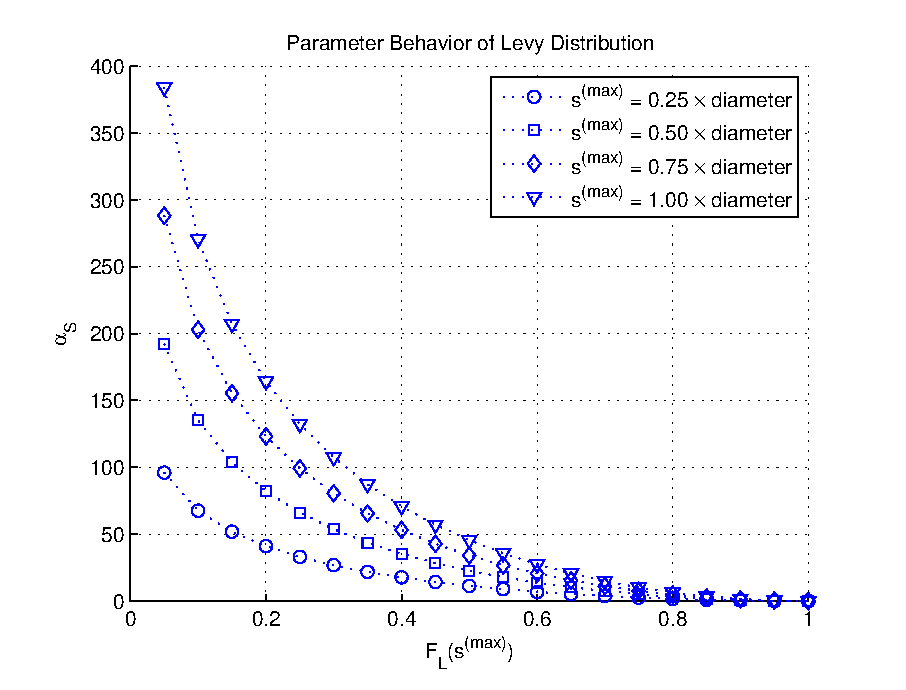
\includegraphics[width=5in]{Chapter_4_Figures/alpha_S.eps}
\caption{$\alpha_S$ behavior of interrogator steps.}
\label{Figure: alpha_S.eps}
\end{figure}
\begin{figure}
\centering
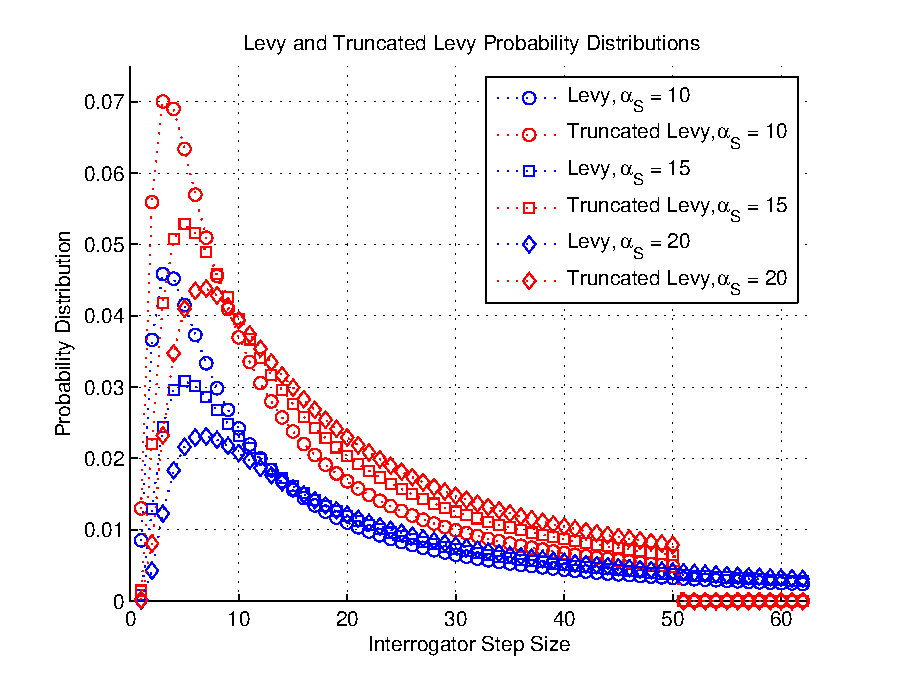
\includegraphics[width=5in]{Chapter_4_Figures/pdf_S.eps}
\caption{PDF of L\'{e}vy and truncated L\'{e}vy distributions.}
\label{Figure: pdf_S.eps}
\end{figure}
\clearpage

\begin{figure}
\centering
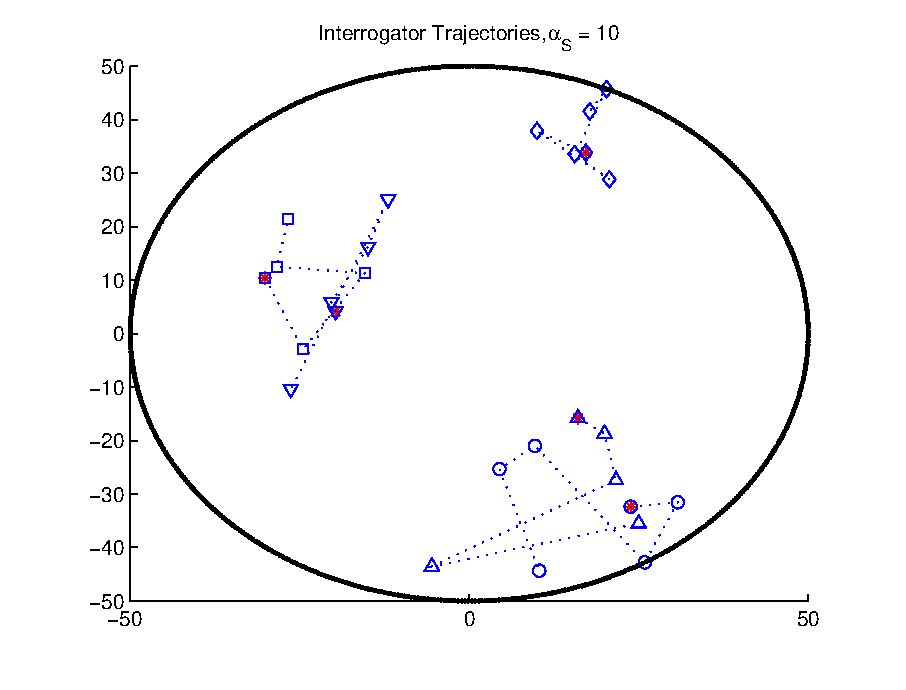
\includegraphics[width=5in]{Chapter_4_Figures/interrogator_traj_alpha_S_10.eps}
\caption{Interrogator trajectories. Number of interrogators $=5$, number of interrogator steps $=4$, and $\alpha_S = 10$.}
\label{Figure: interrogator_traj_alpha_S_10.eps}
\end{figure}
\begin{figure}
\centering
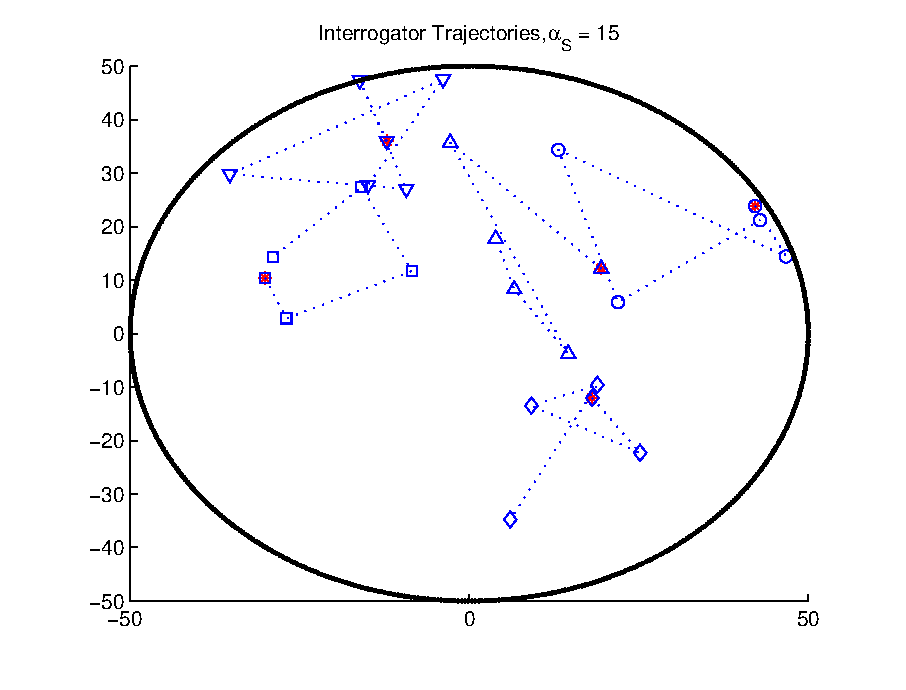
\includegraphics[width=5in]{Chapter_4_Figures/interrogator_traj_alpha_S_15.eps}
\caption{Interrogator trajectories. Number of interrogators $=5$, number of interrogator steps $=4$, and $\alpha_S = 15$.}
\label{Figure: interrogator_traj_alpha_S_15.eps}
\end{figure}
\clearpage

\begin{figure}
\centering
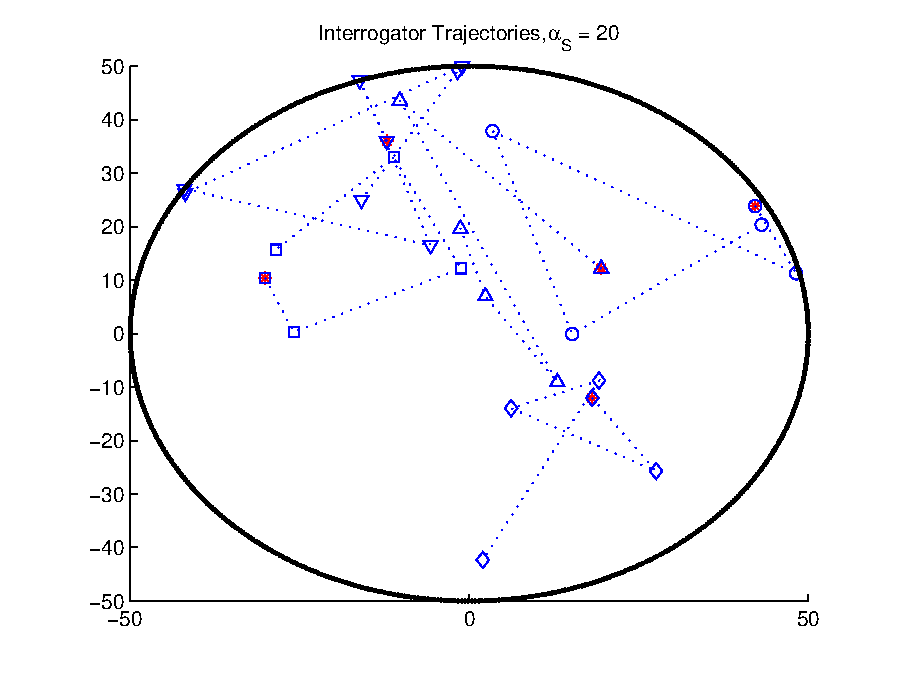
\includegraphics[width=5in]{Chapter_4_Figures/interrogator_traj_alpha_S_20.eps}
\caption{Interrogator trajectories. Number of interrogators $=5$, number of interrogator steps $=4$, and $\alpha_S = 20$.}
\label{Figure: interrogator_traj_alpha_S_20.eps}
\end{figure}
\begin{figure}
\centering
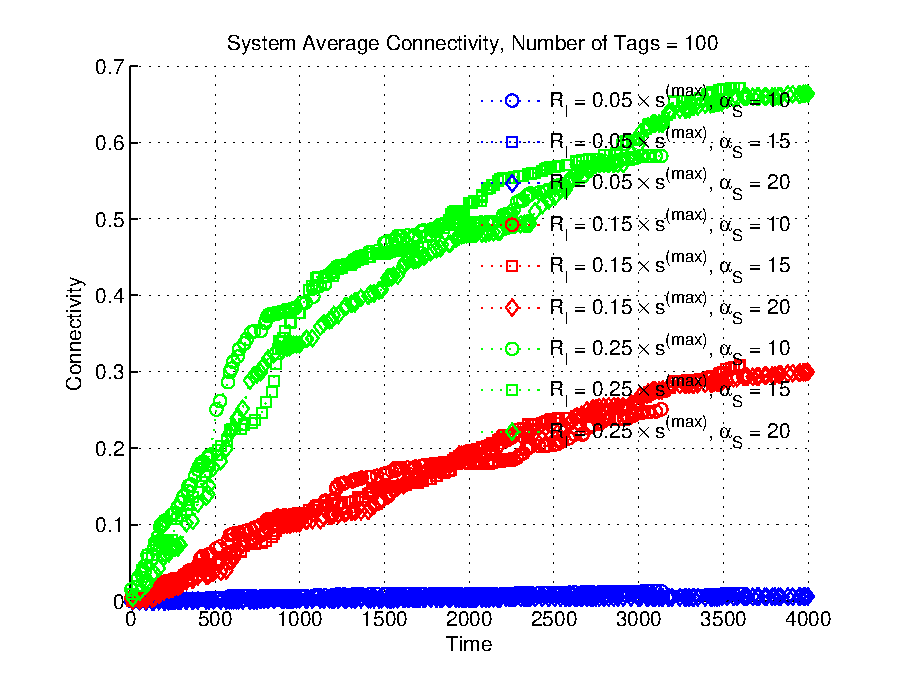
\includegraphics[width=5in]{Chapter_4_Figures/sys_connect_100tags_all.eps}
\caption{System connectivity. Number of tags = 100 and $R_I \in \{0.05, 0.15, 0.25\} \times s^{(max)}$.}
\label{Figure: sys_connect_100tags_all.eps}
\end{figure}
\clearpage

\begin{figure}
\centering
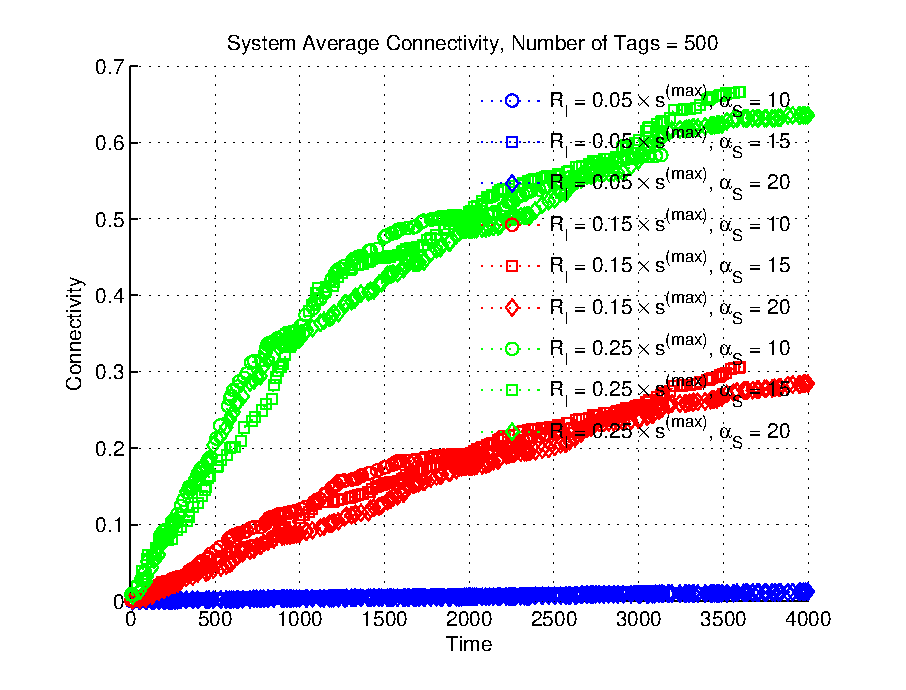
\includegraphics[width=5in]{Chapter_4_Figures/sys_connect_500tags_all.eps}
\caption{System connectivity. Number of tags = 500 and $R_I \in \{0.05, 0.15, 0.25\} \times s^{(max)}$.}
\label{Figure: sys_connect_500tags_all.eps}
\end{figure}
\begin{figure}
\centering
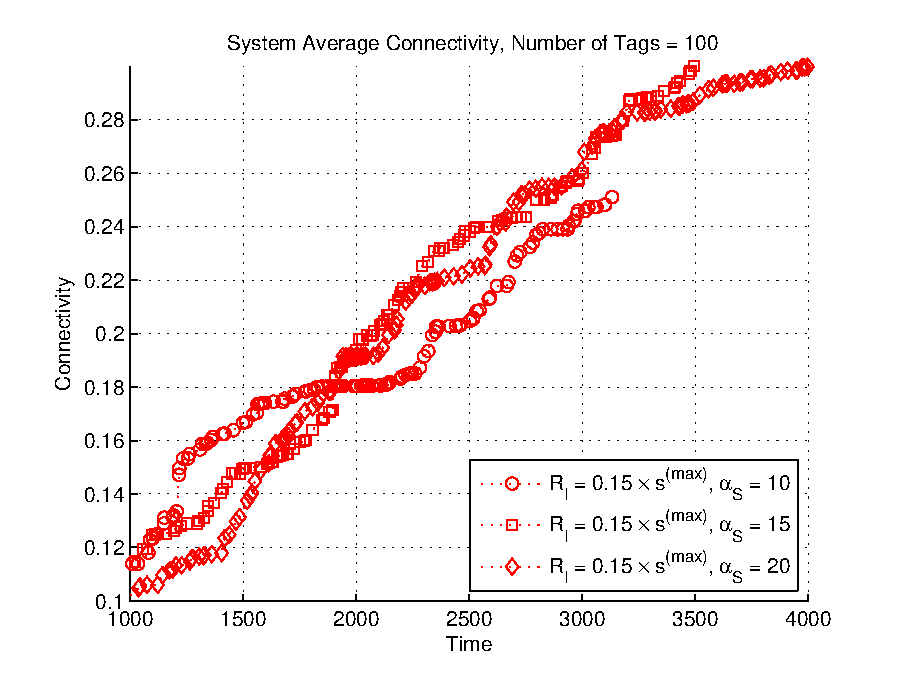
\includegraphics[width=5in]{Chapter_4_Figures/sys_connect_100tags_15diam.eps}
\caption{System connectivity. Number of tags = 100 and $R_I = 0.15 \times s^{(max)}$.}
\label{Figure: sys_connect_100tags_15diam.eps}
\end{figure}
\clearpage

\begin{figure}
\centering
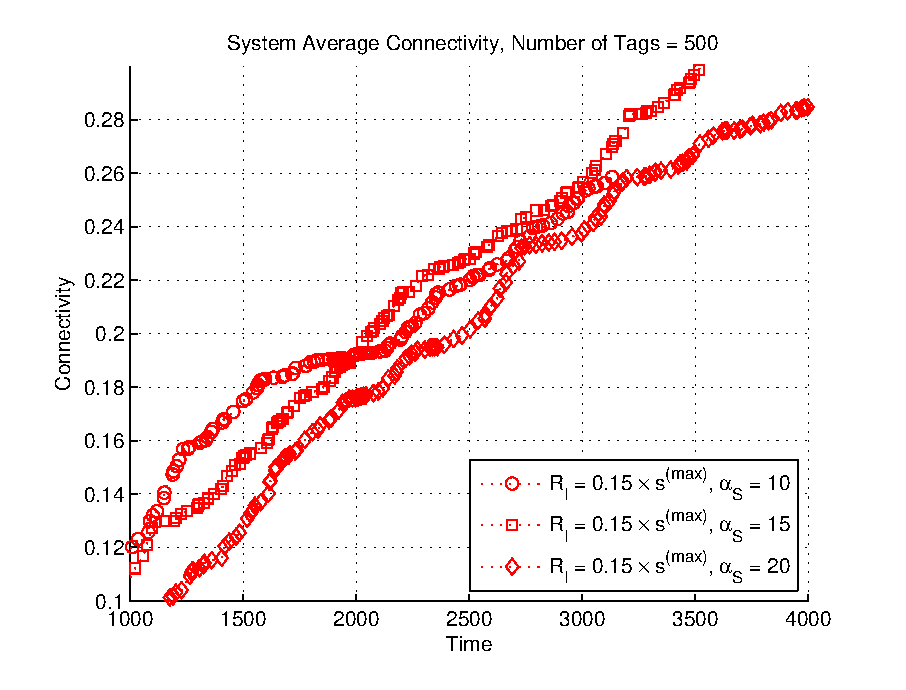
\includegraphics[width=5in]{Chapter_4_Figures/sys_connect_500tags_15diam.eps}
\caption{System connectivity. Number of tags = 500 and $R_I = 0.15 \times s^{(max)}$.}
\label{Figure: sys_connect_500tags_15diam.eps}
\end{figure}
\begin{figure}
\centering
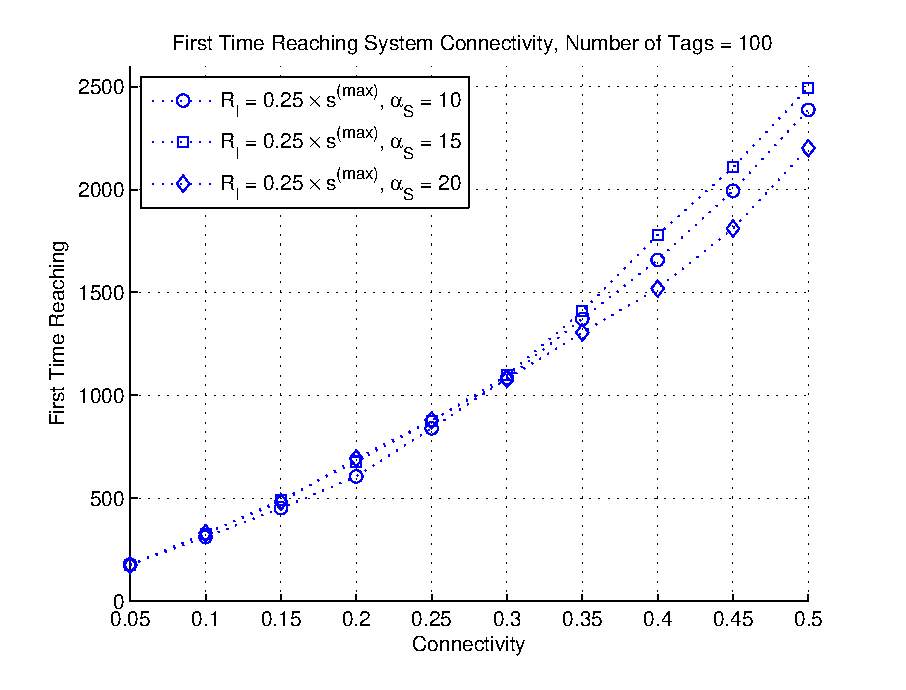
\includegraphics[width=5in]{Chapter_4_Figures/sys_first_time_connect_100tags.eps}
\caption{First time reaching system connectivity. Number of tags = 100 and $R_I \in \{0.05, 0.15, 0.25\} \times s^{(max)}$.}
\label{Figure: sys_first_time_connect_100tags.eps}
\end{figure}
\clearpage

\begin{figure}
\centering
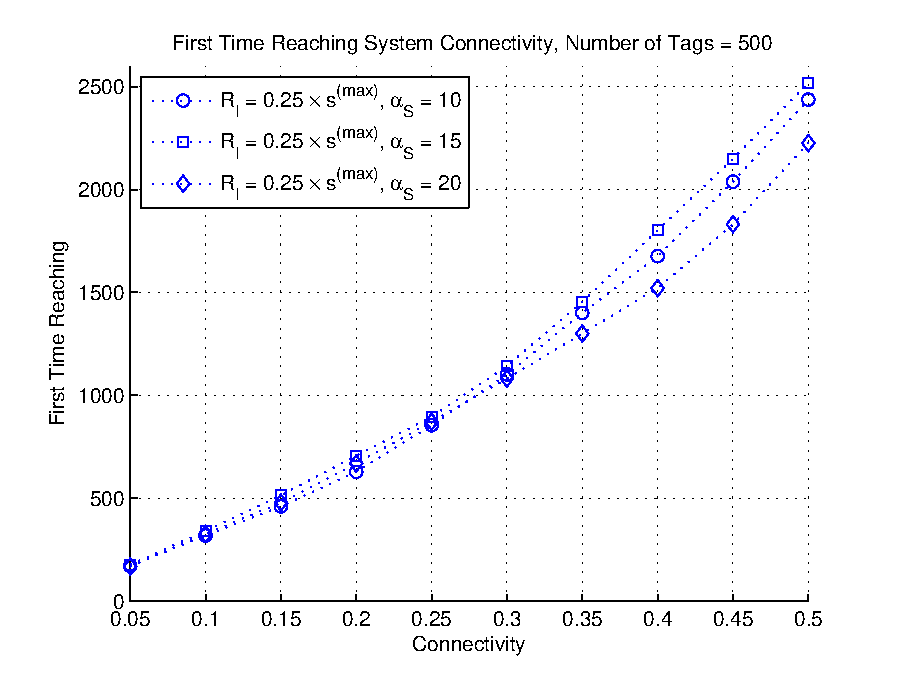
\includegraphics[width=5in]{Chapter_4_Figures/sys_first_time_connect_500tags.eps}
\caption{First time reaching system connectivity. Number of tags = 500 and $R_I \in \{0.05, 0.15, 0.25\} \times s^{(max)}$.}
\label{Figure: sys_first_time_connect_500tags.eps}
\end{figure}
\begin{figure}
\centering
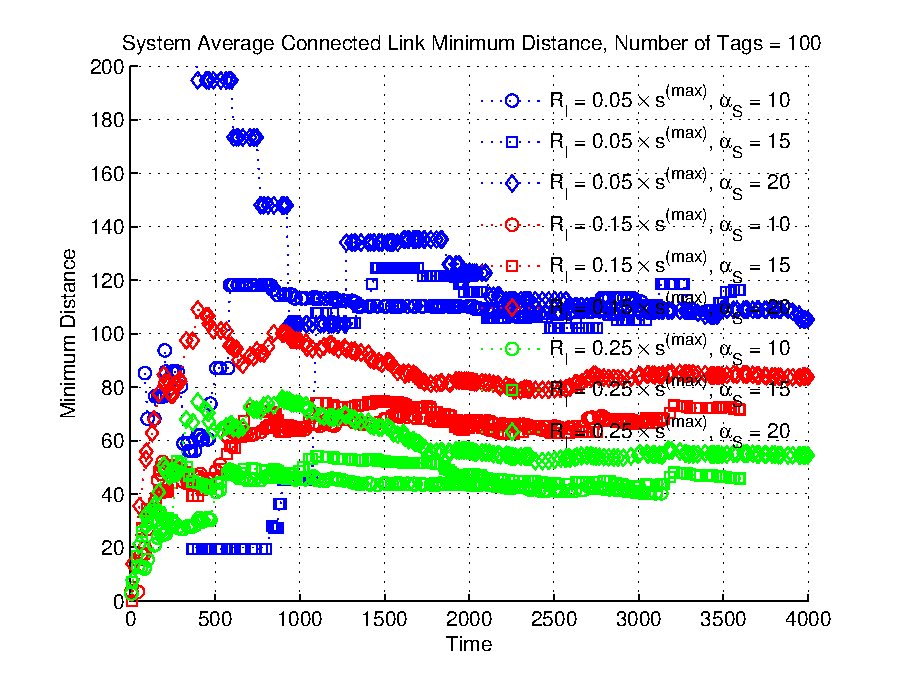
\includegraphics[width=5in]{Chapter_4_Figures/sys_links_min_dist_100tags_all.eps}
\caption{System connected links minimum distances average. Number of tags = 100 and $R_I \in \{0.05, 0.15, 0.25\} \times s^{(max)}$.}
\label{Figure: sys_links_min_dist_100tags_all.eps}
\end{figure}
\clearpage

\begin{figure}
\centering
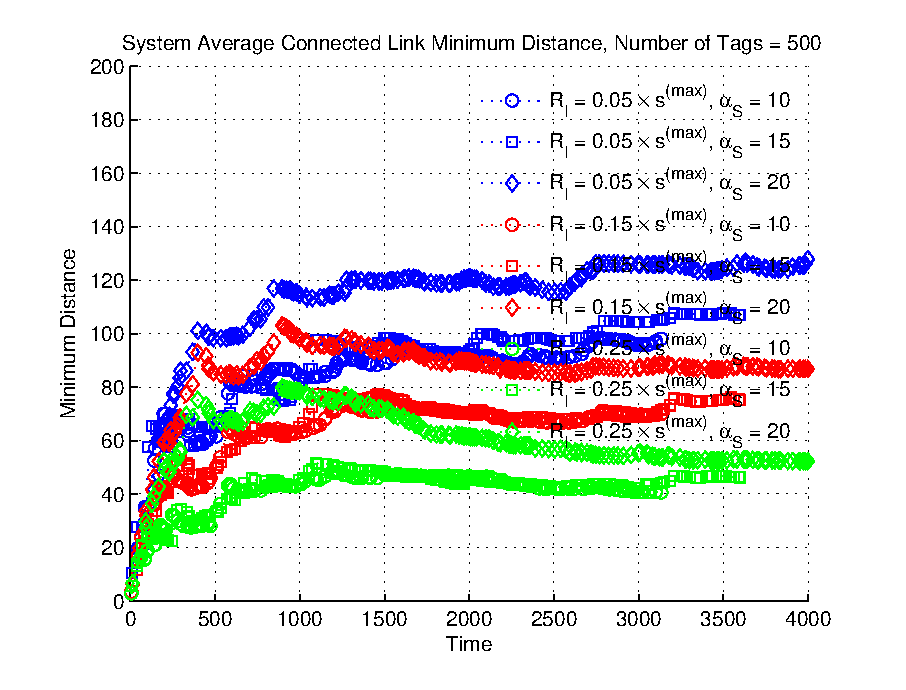
\includegraphics[width=5in]{Chapter_4_Figures/sys_links_min_dist_500tags_all.eps}
\caption{System connected links minimum distances average. Number of tags = 500 and $R_I \in \{0.05, 0.15, 0.25\} \times s^{(max)}$.}
\label{Figure: sys_links_min_dist_500tags_all.eps}
\end{figure}
\begin{figure}
\centering
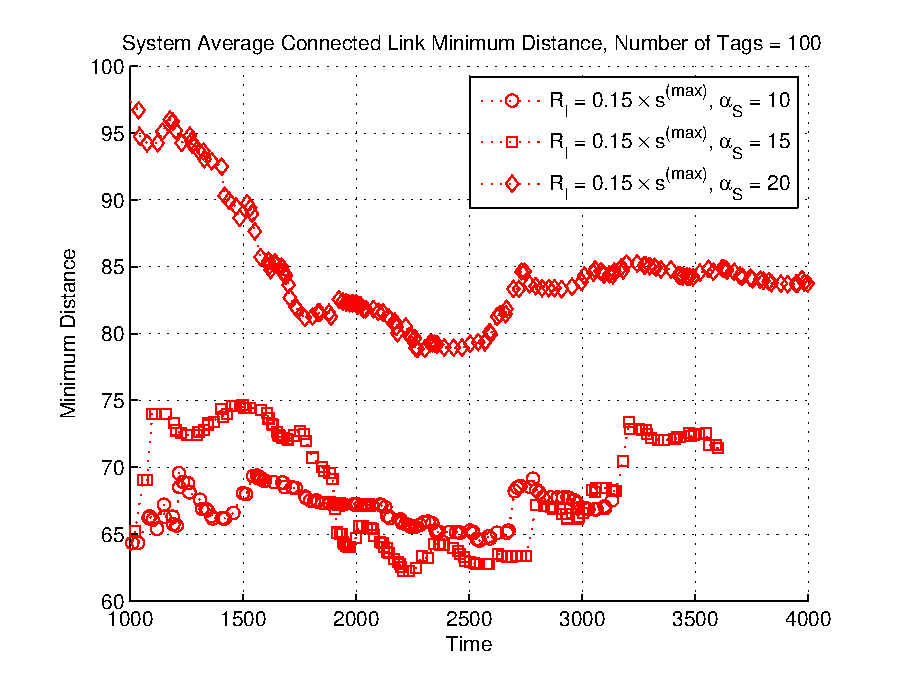
\includegraphics[width=5in]{Chapter_4_Figures/sys_links_min_dist_100tags_15diam.eps}
\caption{System connected links minimum distances average. Number of tags = 100 and $R_I = 0.15 \times s^{(max)}$.}
\label{Figure: sys_links_min_dist_100tags_15diam.eps}
\end{figure}
\clearpage

\begin{figure}
\centering
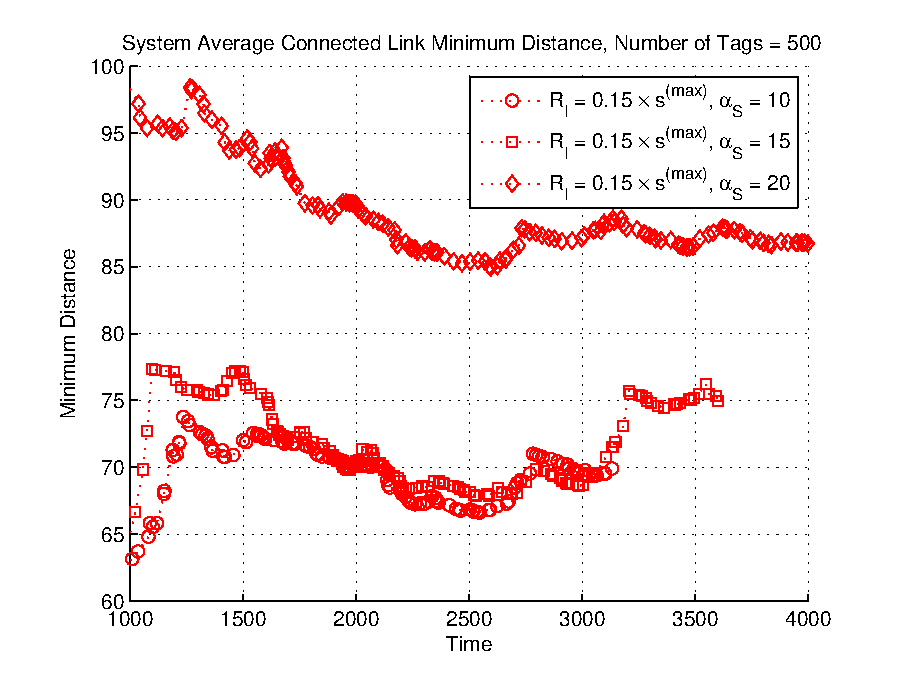
\includegraphics[width=5in]{Chapter_4_Figures/sys_links_min_dist_500tags_15diam.eps}
\caption{System connected links minimum distances average. Number of tags = 500 and $R_I = 0.15 \times s^{(max)}$.}
\label{Figure: sys_links_min_dist_500tags_15diam.eps}
\end{figure}
\begin{figure}
\centering
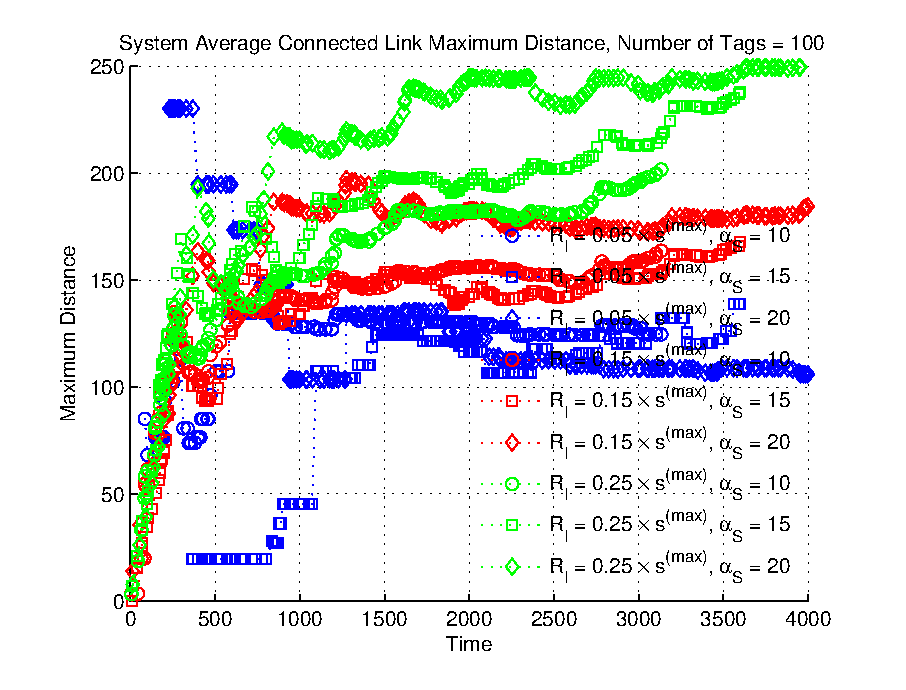
\includegraphics[width=5in]{Chapter_4_Figures/sys_links_max_dist_100tags_all.eps}
\caption{System connected links maximum distances average. Number of tags = 100 and $R_I \in \{0.05, 0.15, 0.25\} \times s^{(max)}$.}
\label{Figure: sys_links_max_dist_100tags_all.eps}
\end{figure}
\clearpage

\begin{figure}
\centering
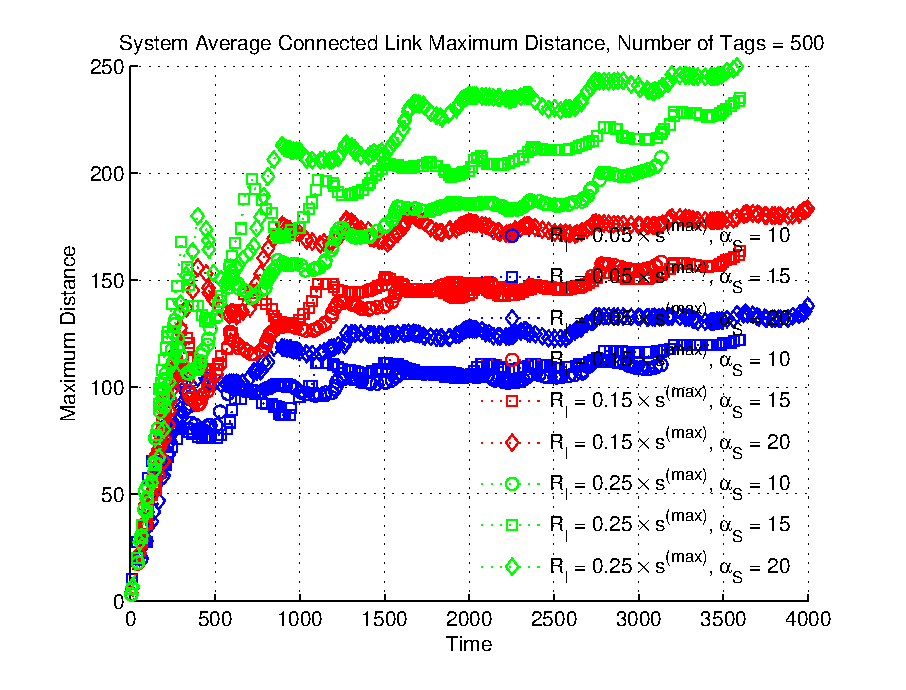
\includegraphics[width=5in]{Chapter_4_Figures/sys_links_max_dist_500tags_all.eps}
\caption{System connected links maximum distances average. Number of tags = 500 and $R_I \in \{0.05, 0.15, 0.25\} \times s^{(max)}$.}
\label{Figure: sys_links_max_dist_500tags_all.eps}
\end{figure}
\begin{figure}
\centering
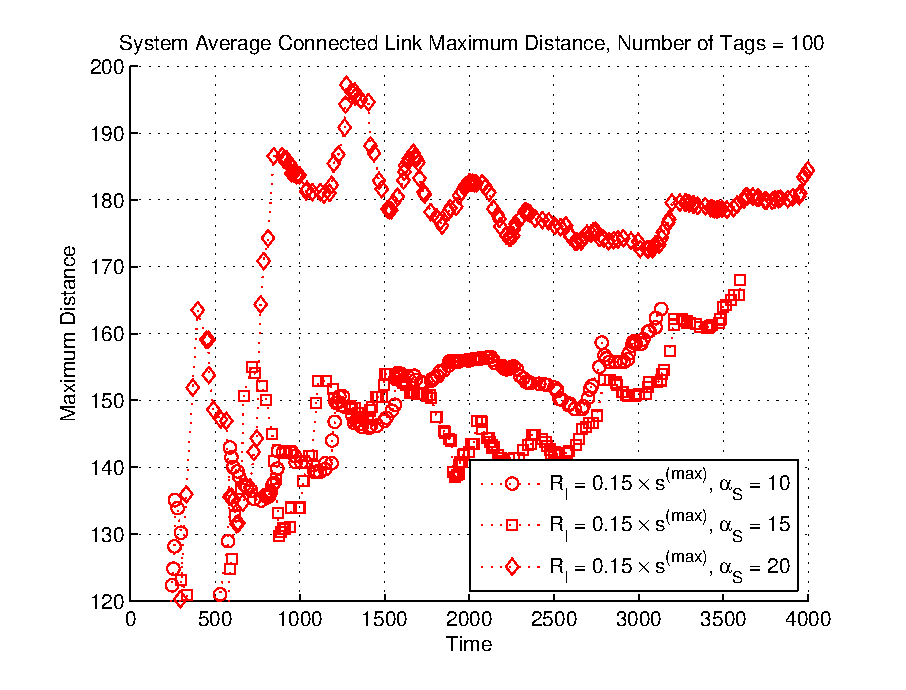
\includegraphics[width=5in]{Chapter_4_Figures/sys_links_max_dist_100tags_15diam.eps}
\caption{System connected links maximum distances average. Number of tags = 100 and $R_I = 0.15 \times s^{(max)}$.}
\label{Figure: sys_links_max_dist_100tags_15diam.eps}
\end{figure}
\clearpage

\begin{figure}
\centering
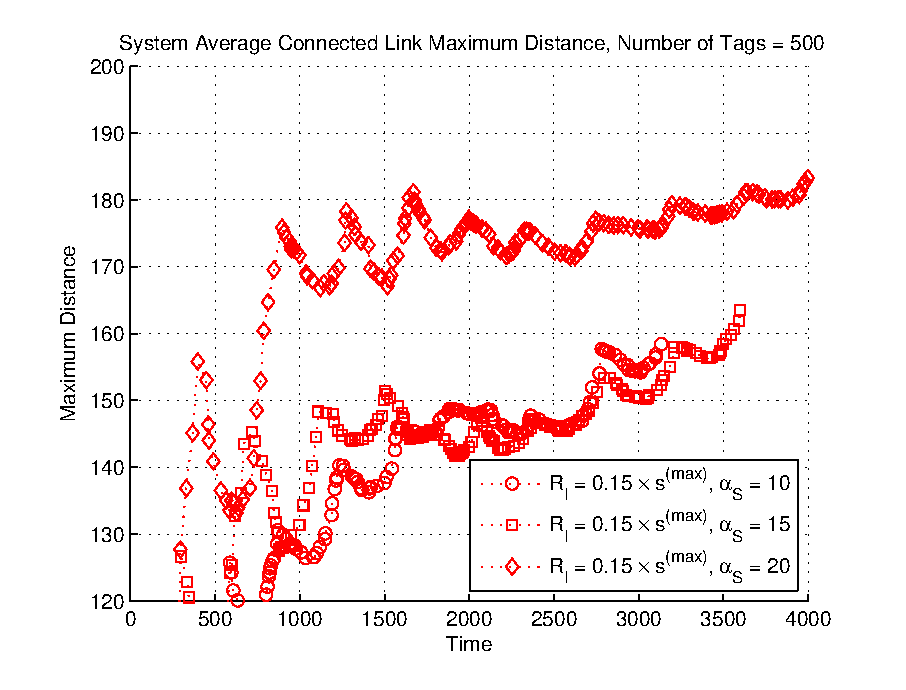
\includegraphics[width=5in]{Chapter_4_Figures/sys_links_max_dist_500tags_15diam.eps}
\caption{System connected links maximum distances average. Number of tags = 500 and $R_I = 0.15 \times s^{(max)}$.}
\label{Figure: sys_links_max_dist_500tags_15diam.eps}
\end{figure}
\begin{figure}
\centering
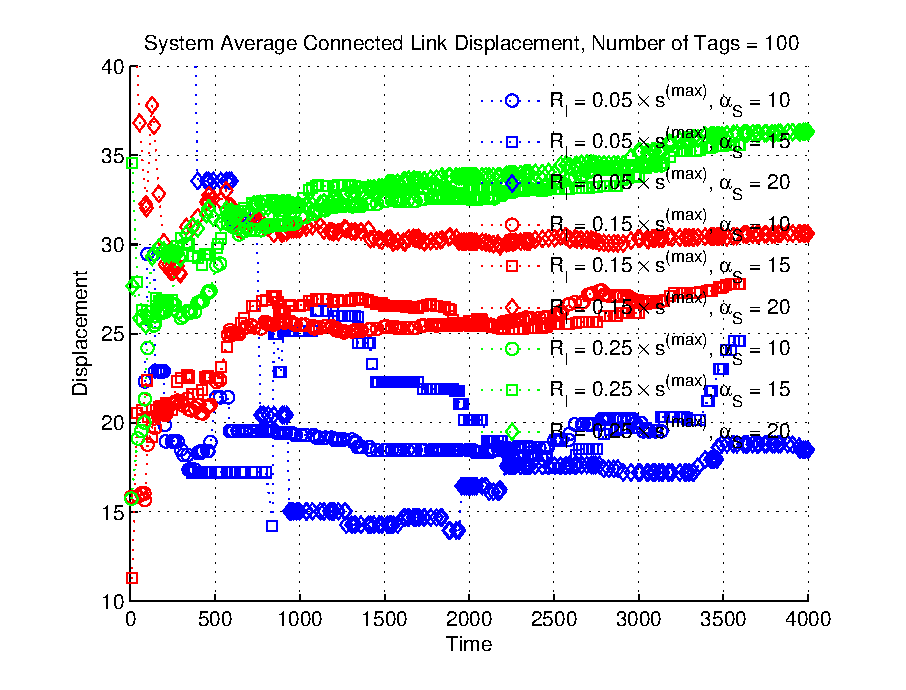
\includegraphics[width=5in]{Chapter_4_Figures/sys_links_disp_100tags_all.eps}
\caption{System connected links displacements average. Number of tags = 100 and $R_I \in \{0.05, 0.15, 0.25\} \times s^{(max)}$.}
\label{Figure: sys_links_disp_100tags_all.eps}
\end{figure}
\clearpage

\begin{figure}
\centering
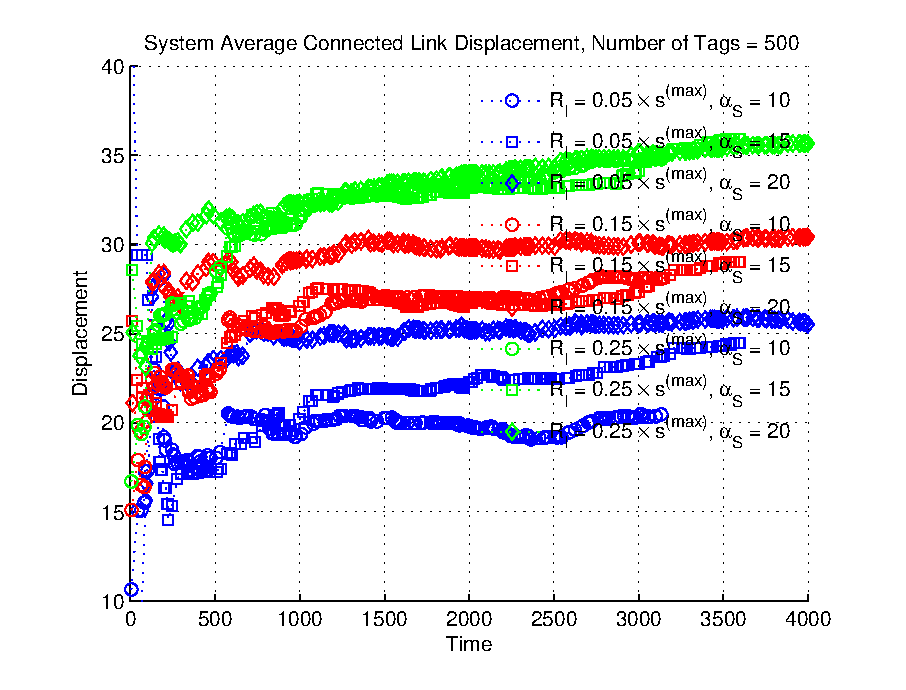
\includegraphics[width=5in]{Chapter_4_Figures/sys_links_disp_500tags_all.eps}
\caption{System connected links displacements average. Number of tags = 500 and $R_I \in \{0.05, 0.15, 0.25\} \times s^{(max)}$.}
\label{Figure: sys_links_disp_500tags_all.eps}
\end{figure}
\begin{figure}
\centering
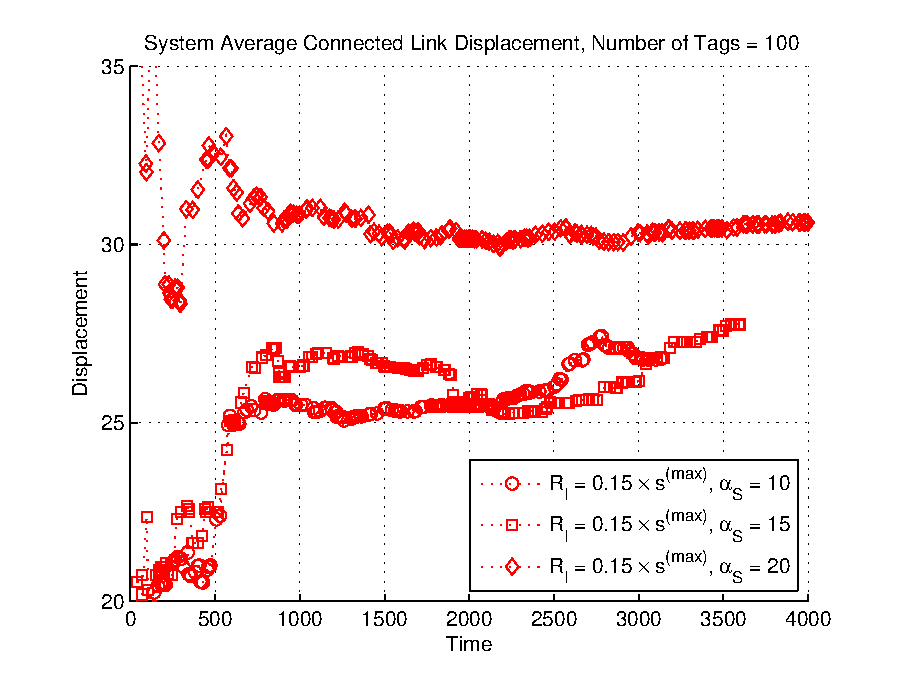
\includegraphics[width=5in]{Chapter_4_Figures/sys_links_disp_100tags_15diam.eps}
\caption{System connected links displacements average. Number of tags = 100 and $R_I = 0.15 \times s^{(max)}$.}
\label{Figure: sys_links_disp_100tags_15diam.eps}
\end{figure}
\clearpage

\begin{figure}
\centering
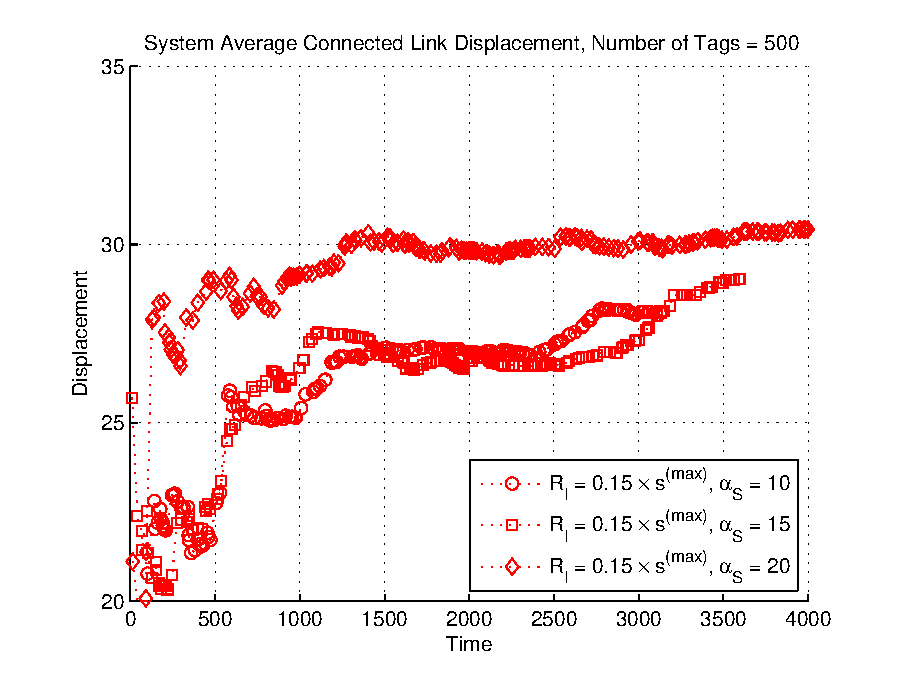
\includegraphics[width=5in]{Chapter_4_Figures/sys_links_disp_500tags_15diam.eps}
\caption{System connected links displacements average. Number of tags = 500 and $R_I = 0.15 \times s^{(max)}$.}
\label{Figure: sys_links_disp_500tags_15diam.eps}
\end{figure}
\begin{figure}
\centering
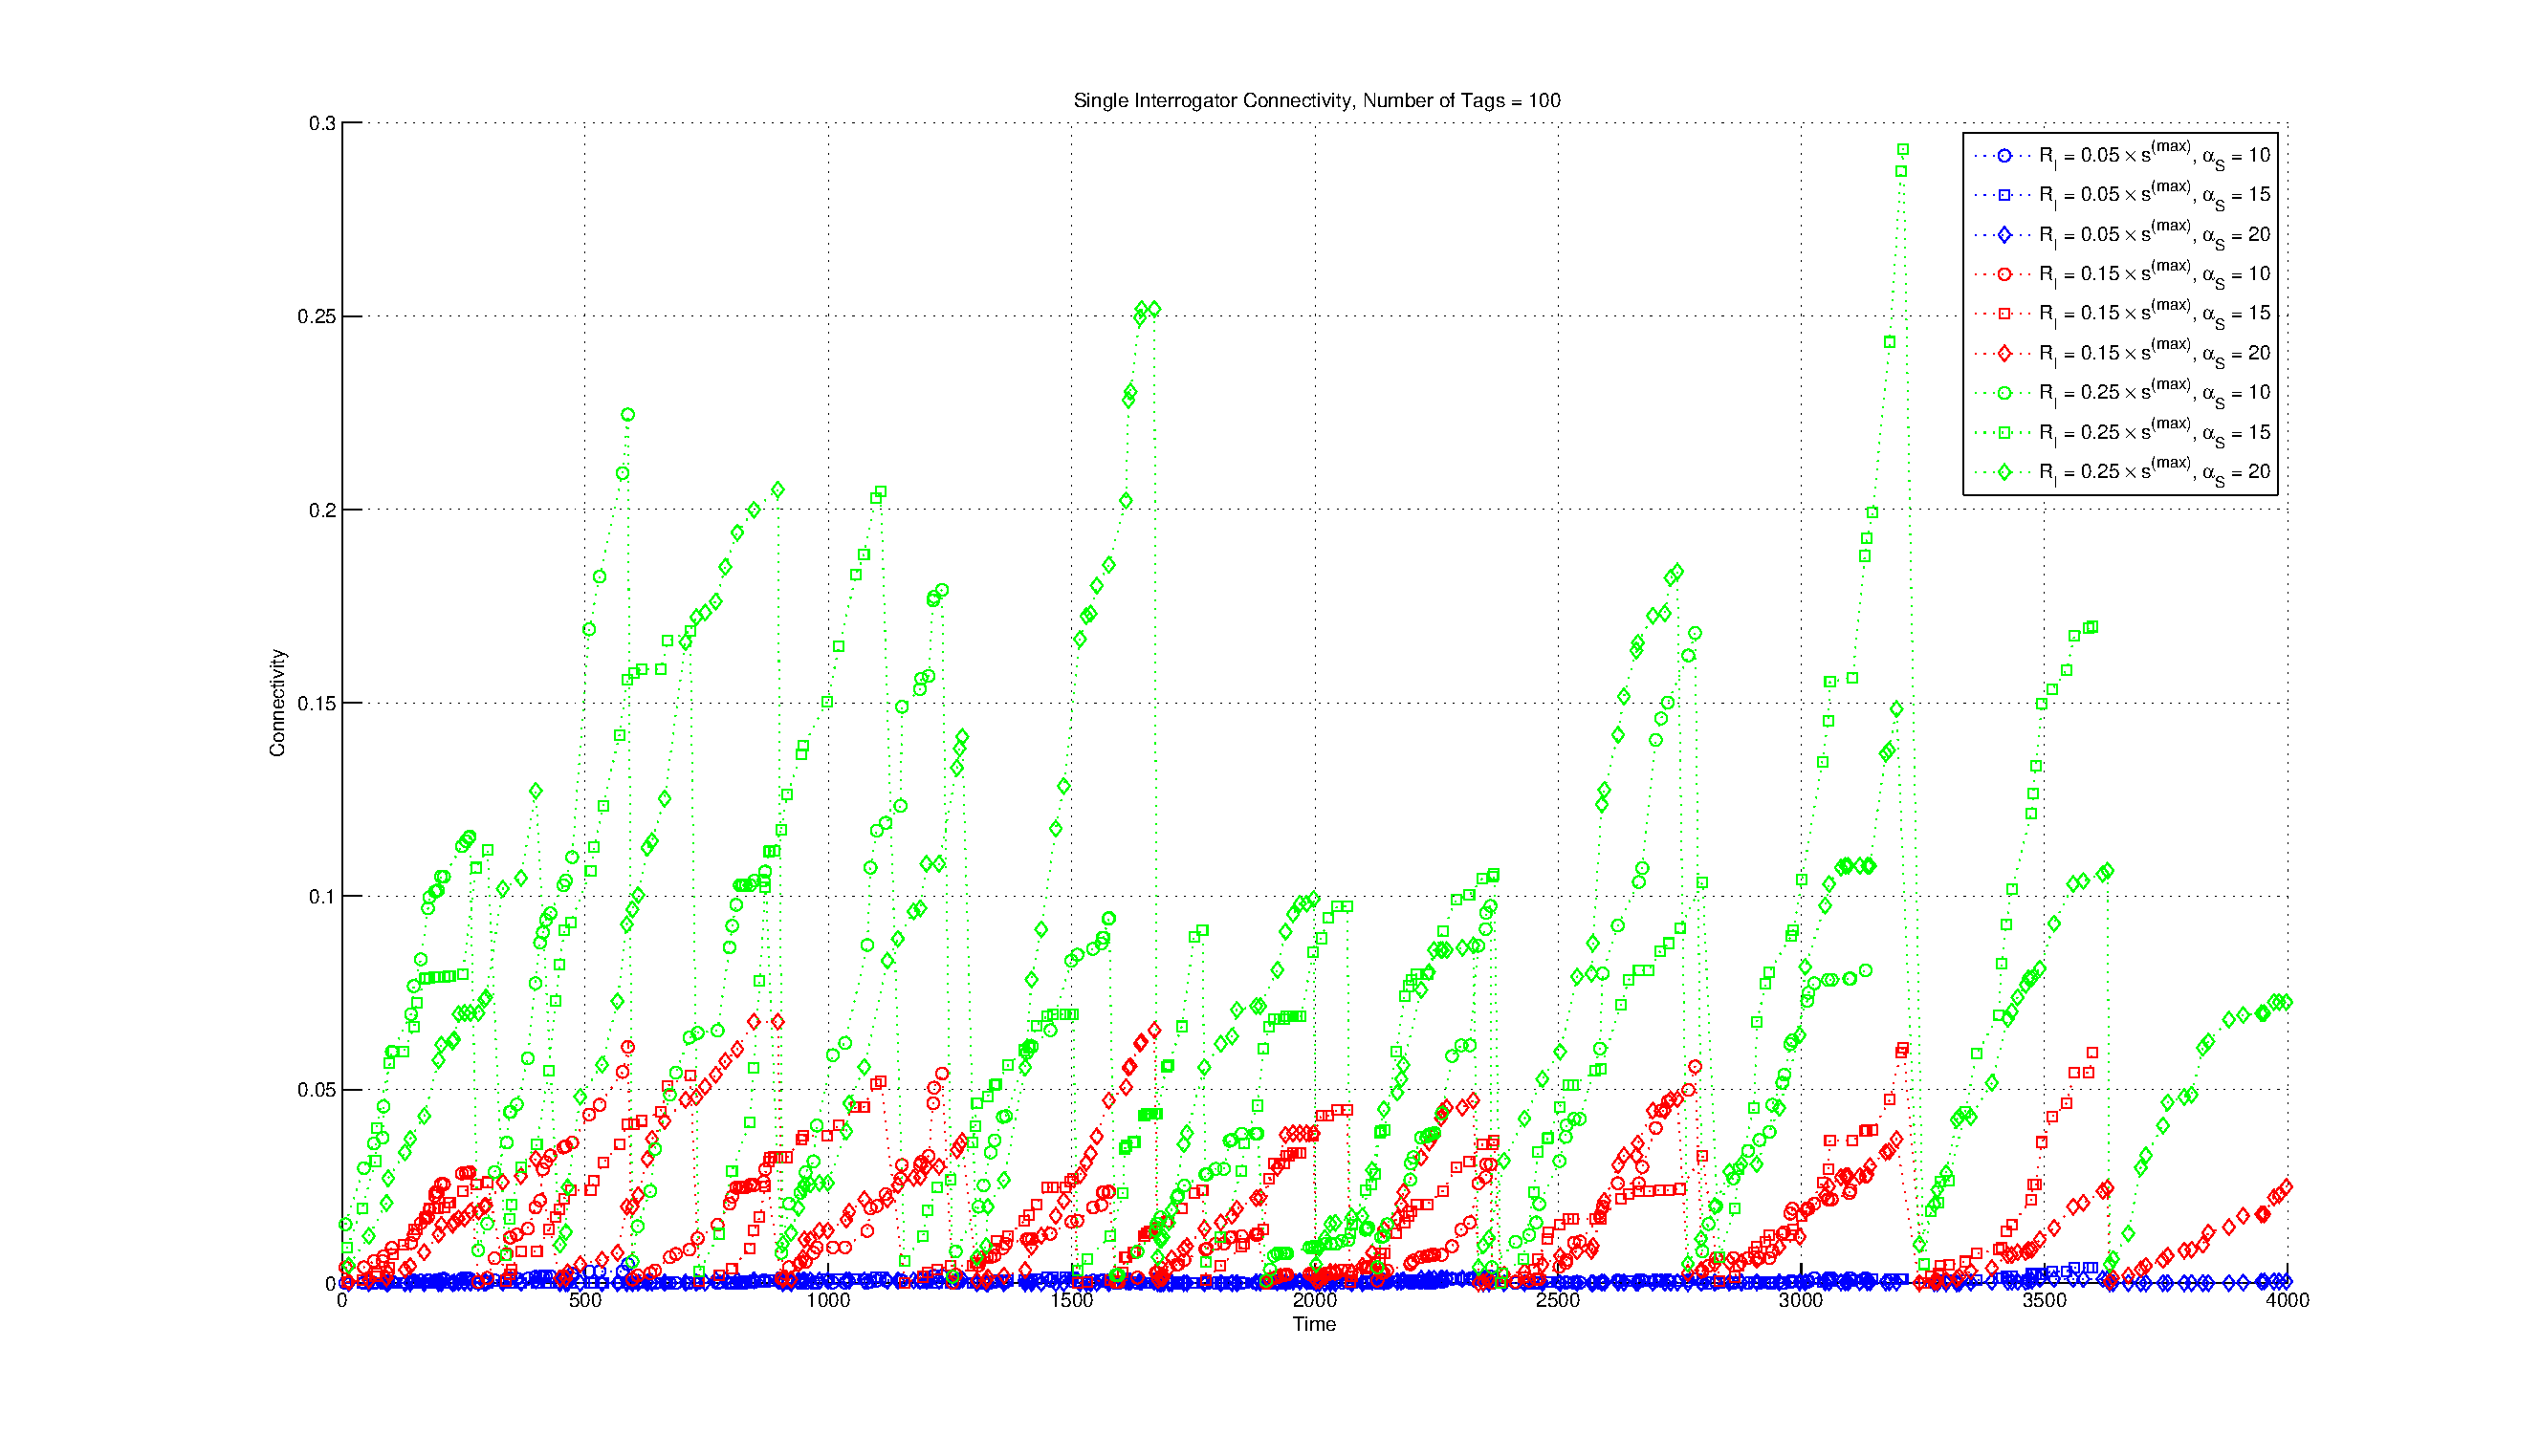
\includegraphics[width=5in, height=3.5in]{Chapter_4_Figures/sin_connect_100tags_all.eps}
\caption{Single interrogator connectivity. Number of tags = 100 and $R_I \in \{0.05, 0.15, 0.25\} \times s^{(max)}$.}
\label{Figure: sin_connect_100tags_all.eps}
\end{figure}
\clearpage

\begin{figure}
\centering
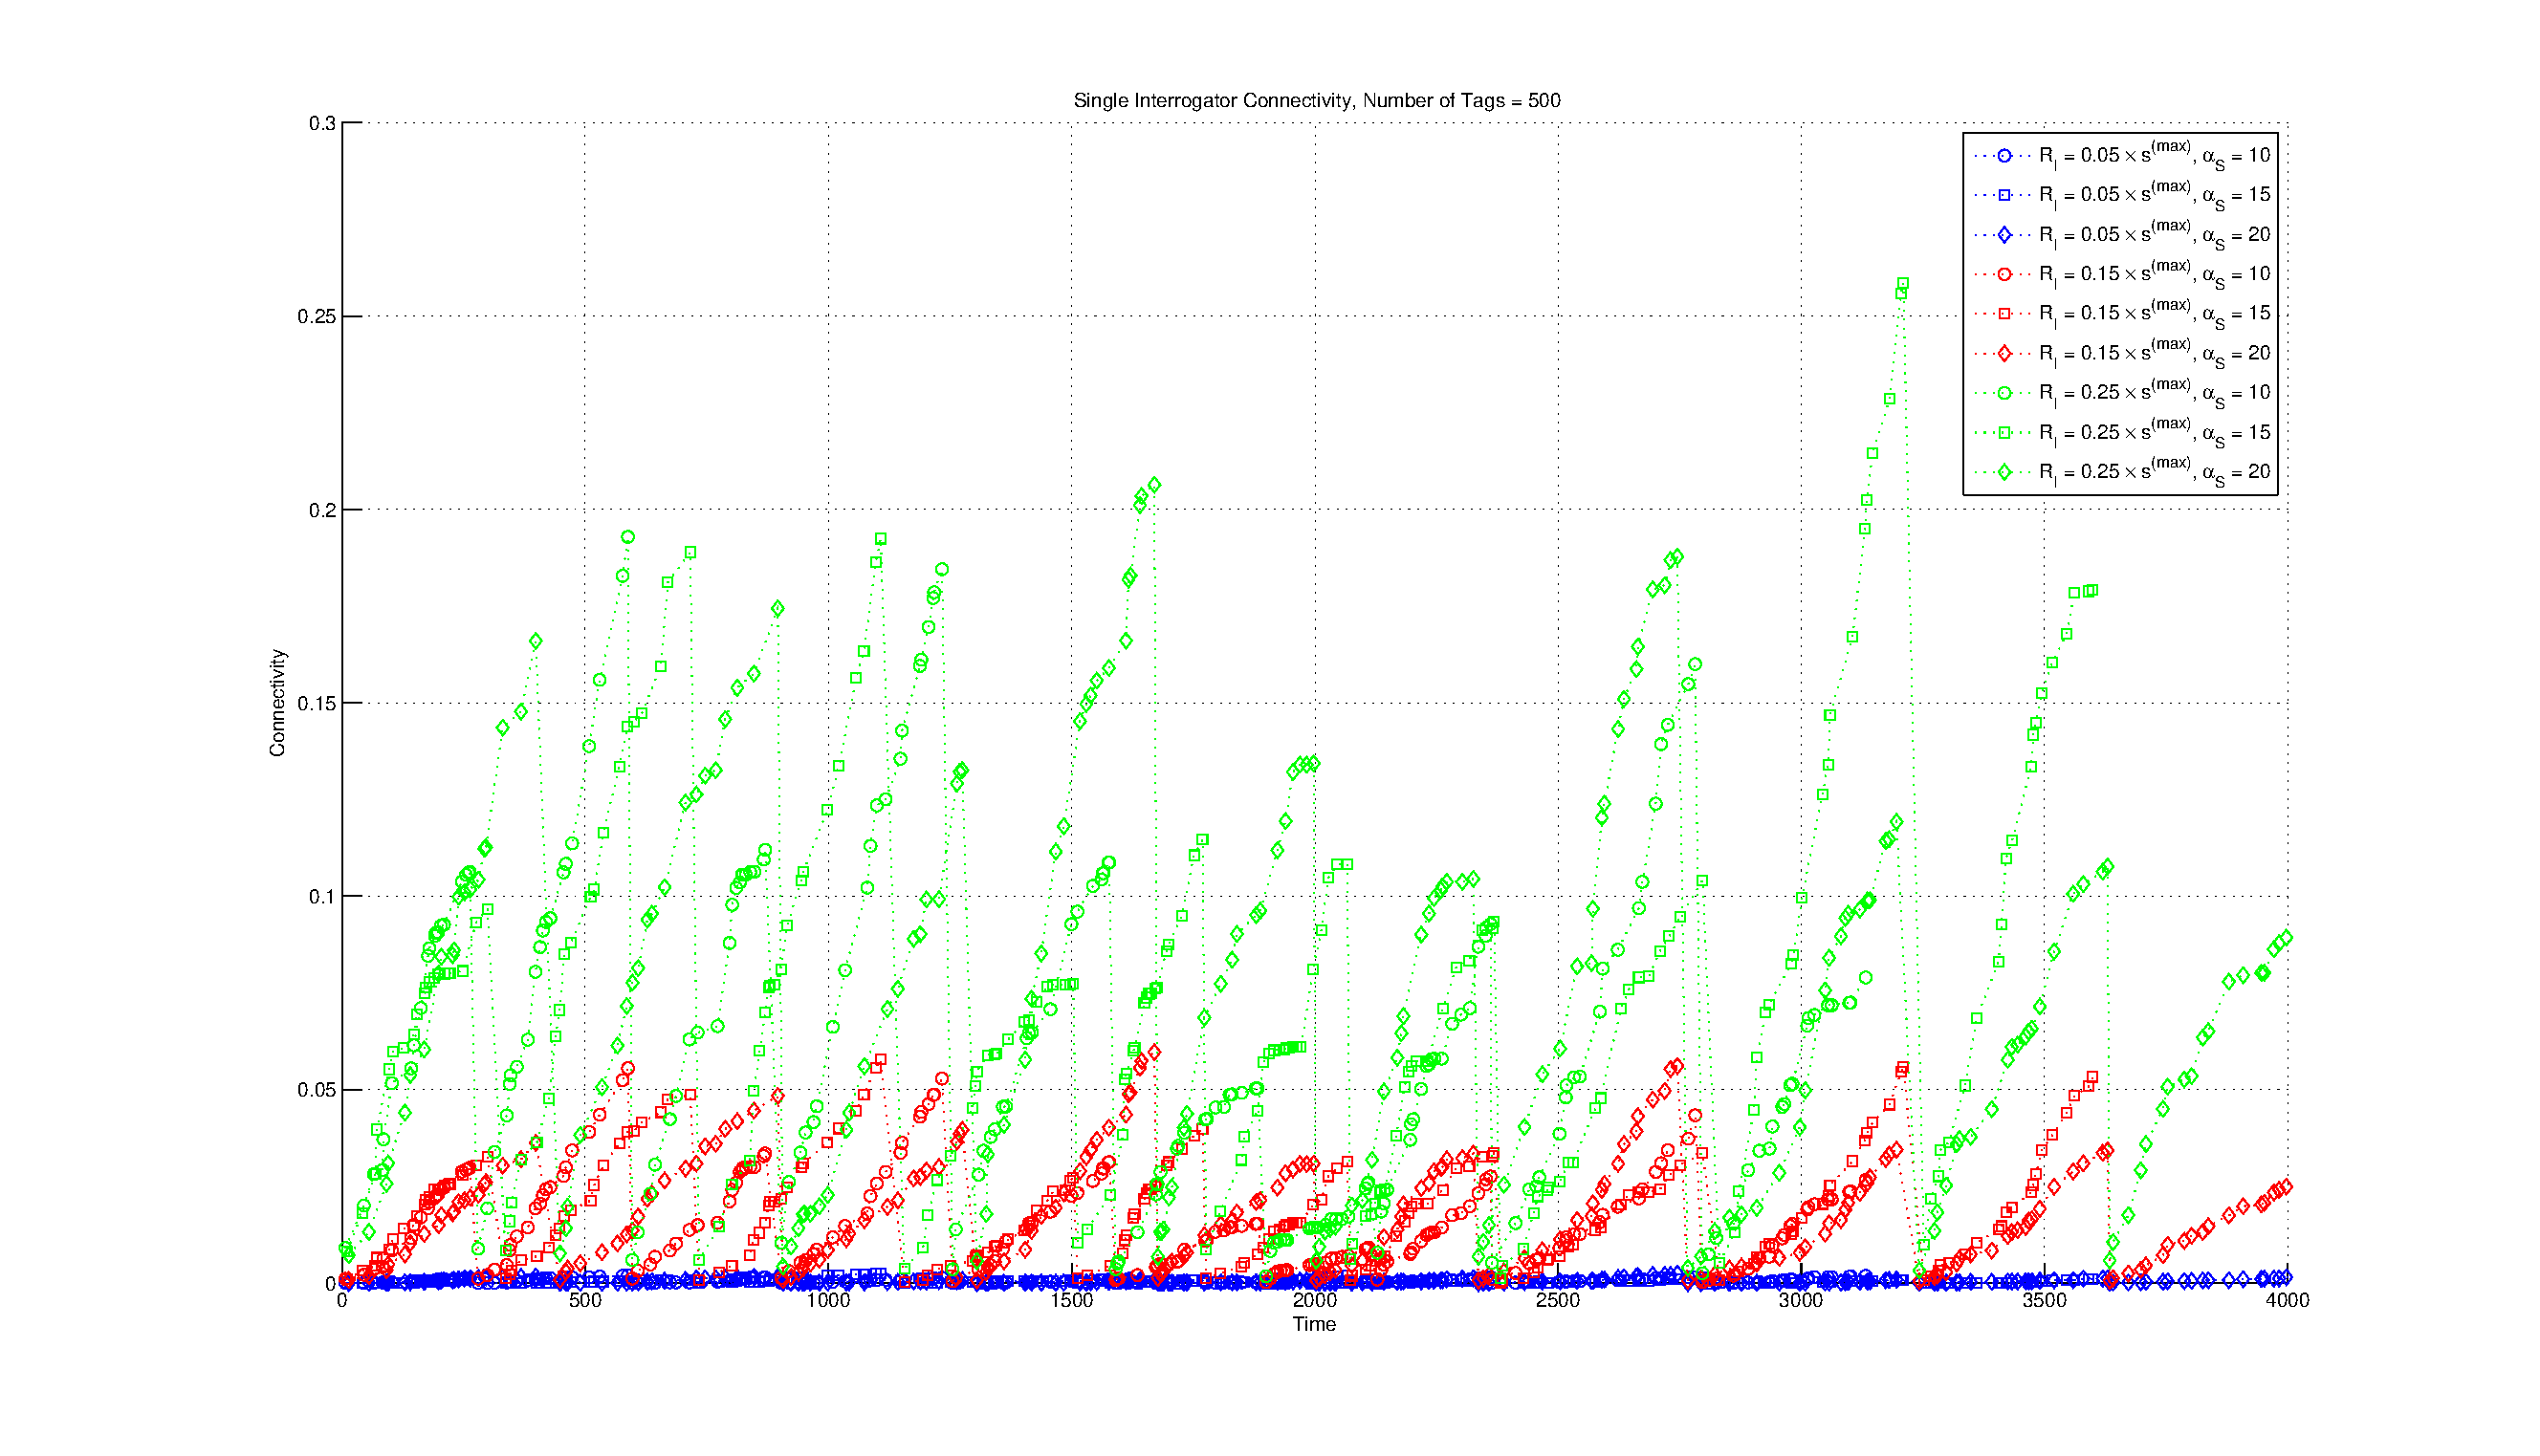
\includegraphics[width=5in, height=3.5in]{Chapter_4_Figures/sin_connect_500tags_all.eps}
\caption{Single interrogator connectivity. Number of tags = 500 and $R_I \in \{0.05, 0.15, 0.25\} \times s^{(max)}$.}
\label{Figure: sin_connect_500tags_all.eps}
\end{figure}
\begin{figure}
\centering
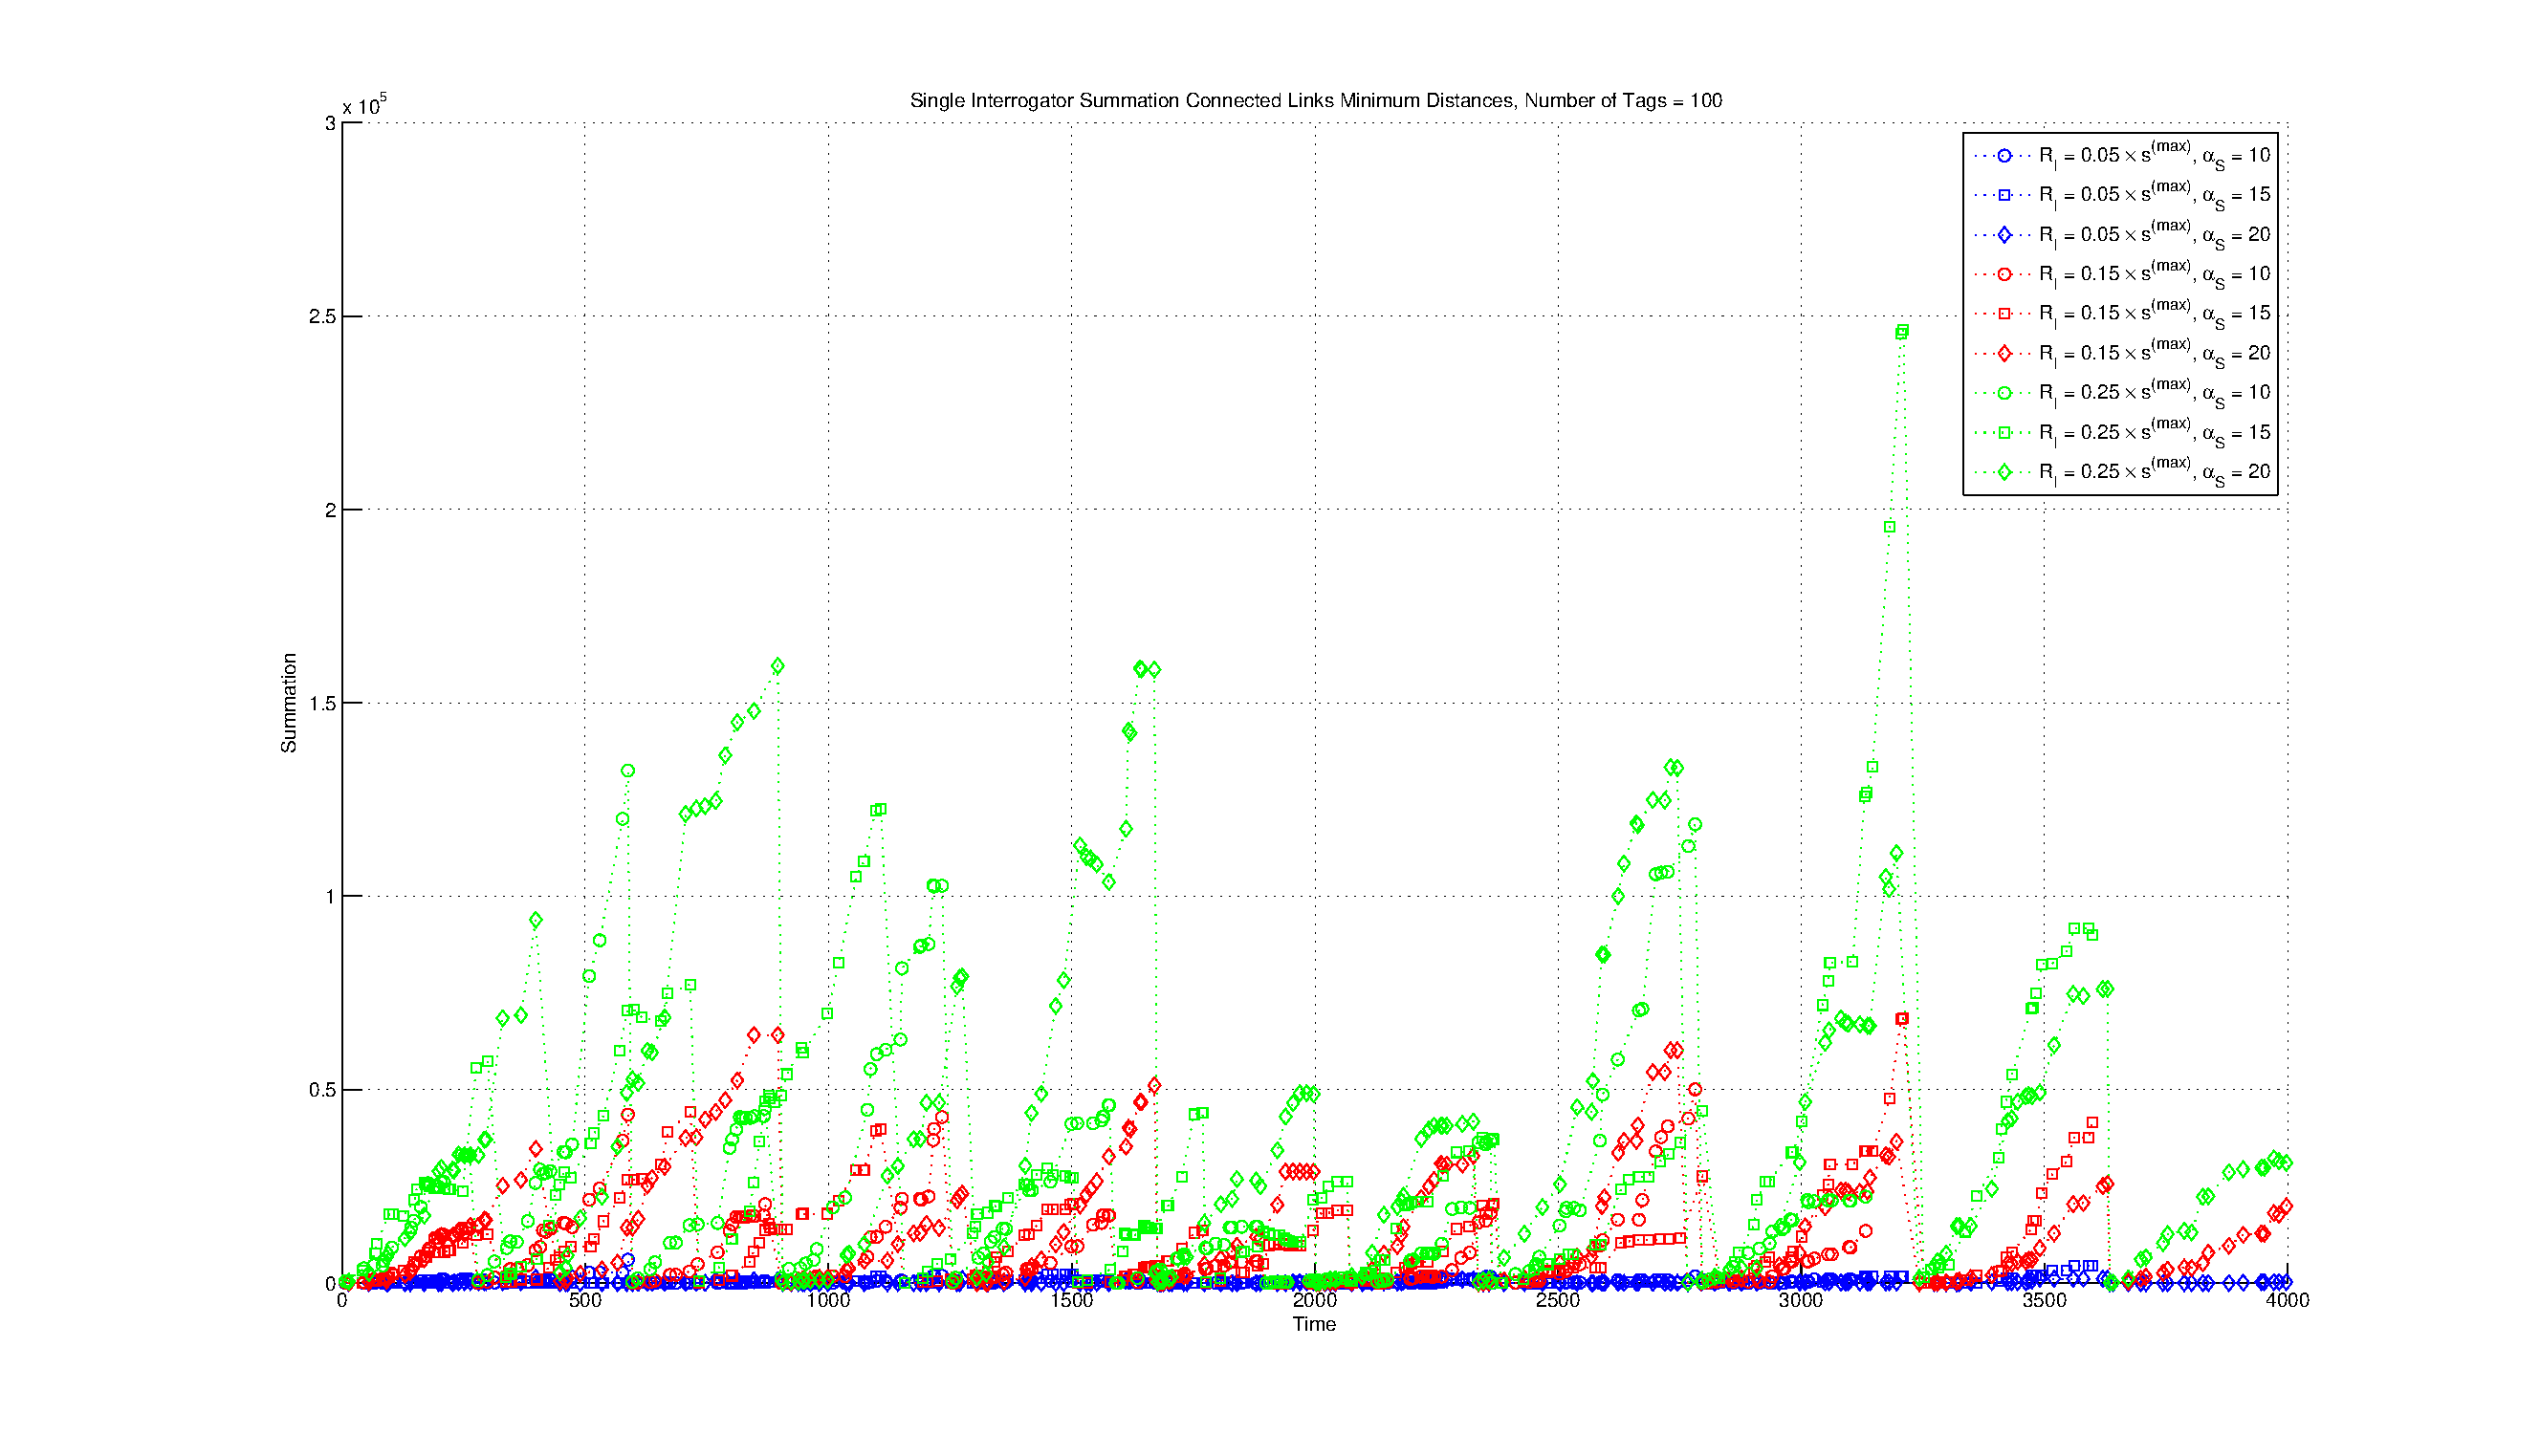
\includegraphics[width=5in, height=3.5in]{Chapter_4_Figures/sin_min_100tags_all.eps}
\caption{Single interrogator summation of connected links minimum distances. Number of tags = 100 and $R_I \in \{0.05, 0.15, 0.25\} \times s^{(max)}$.}
\label{Figure: sin_min_100tags_all.eps}
\end{figure}
\clearpage

\begin{figure}
\centering
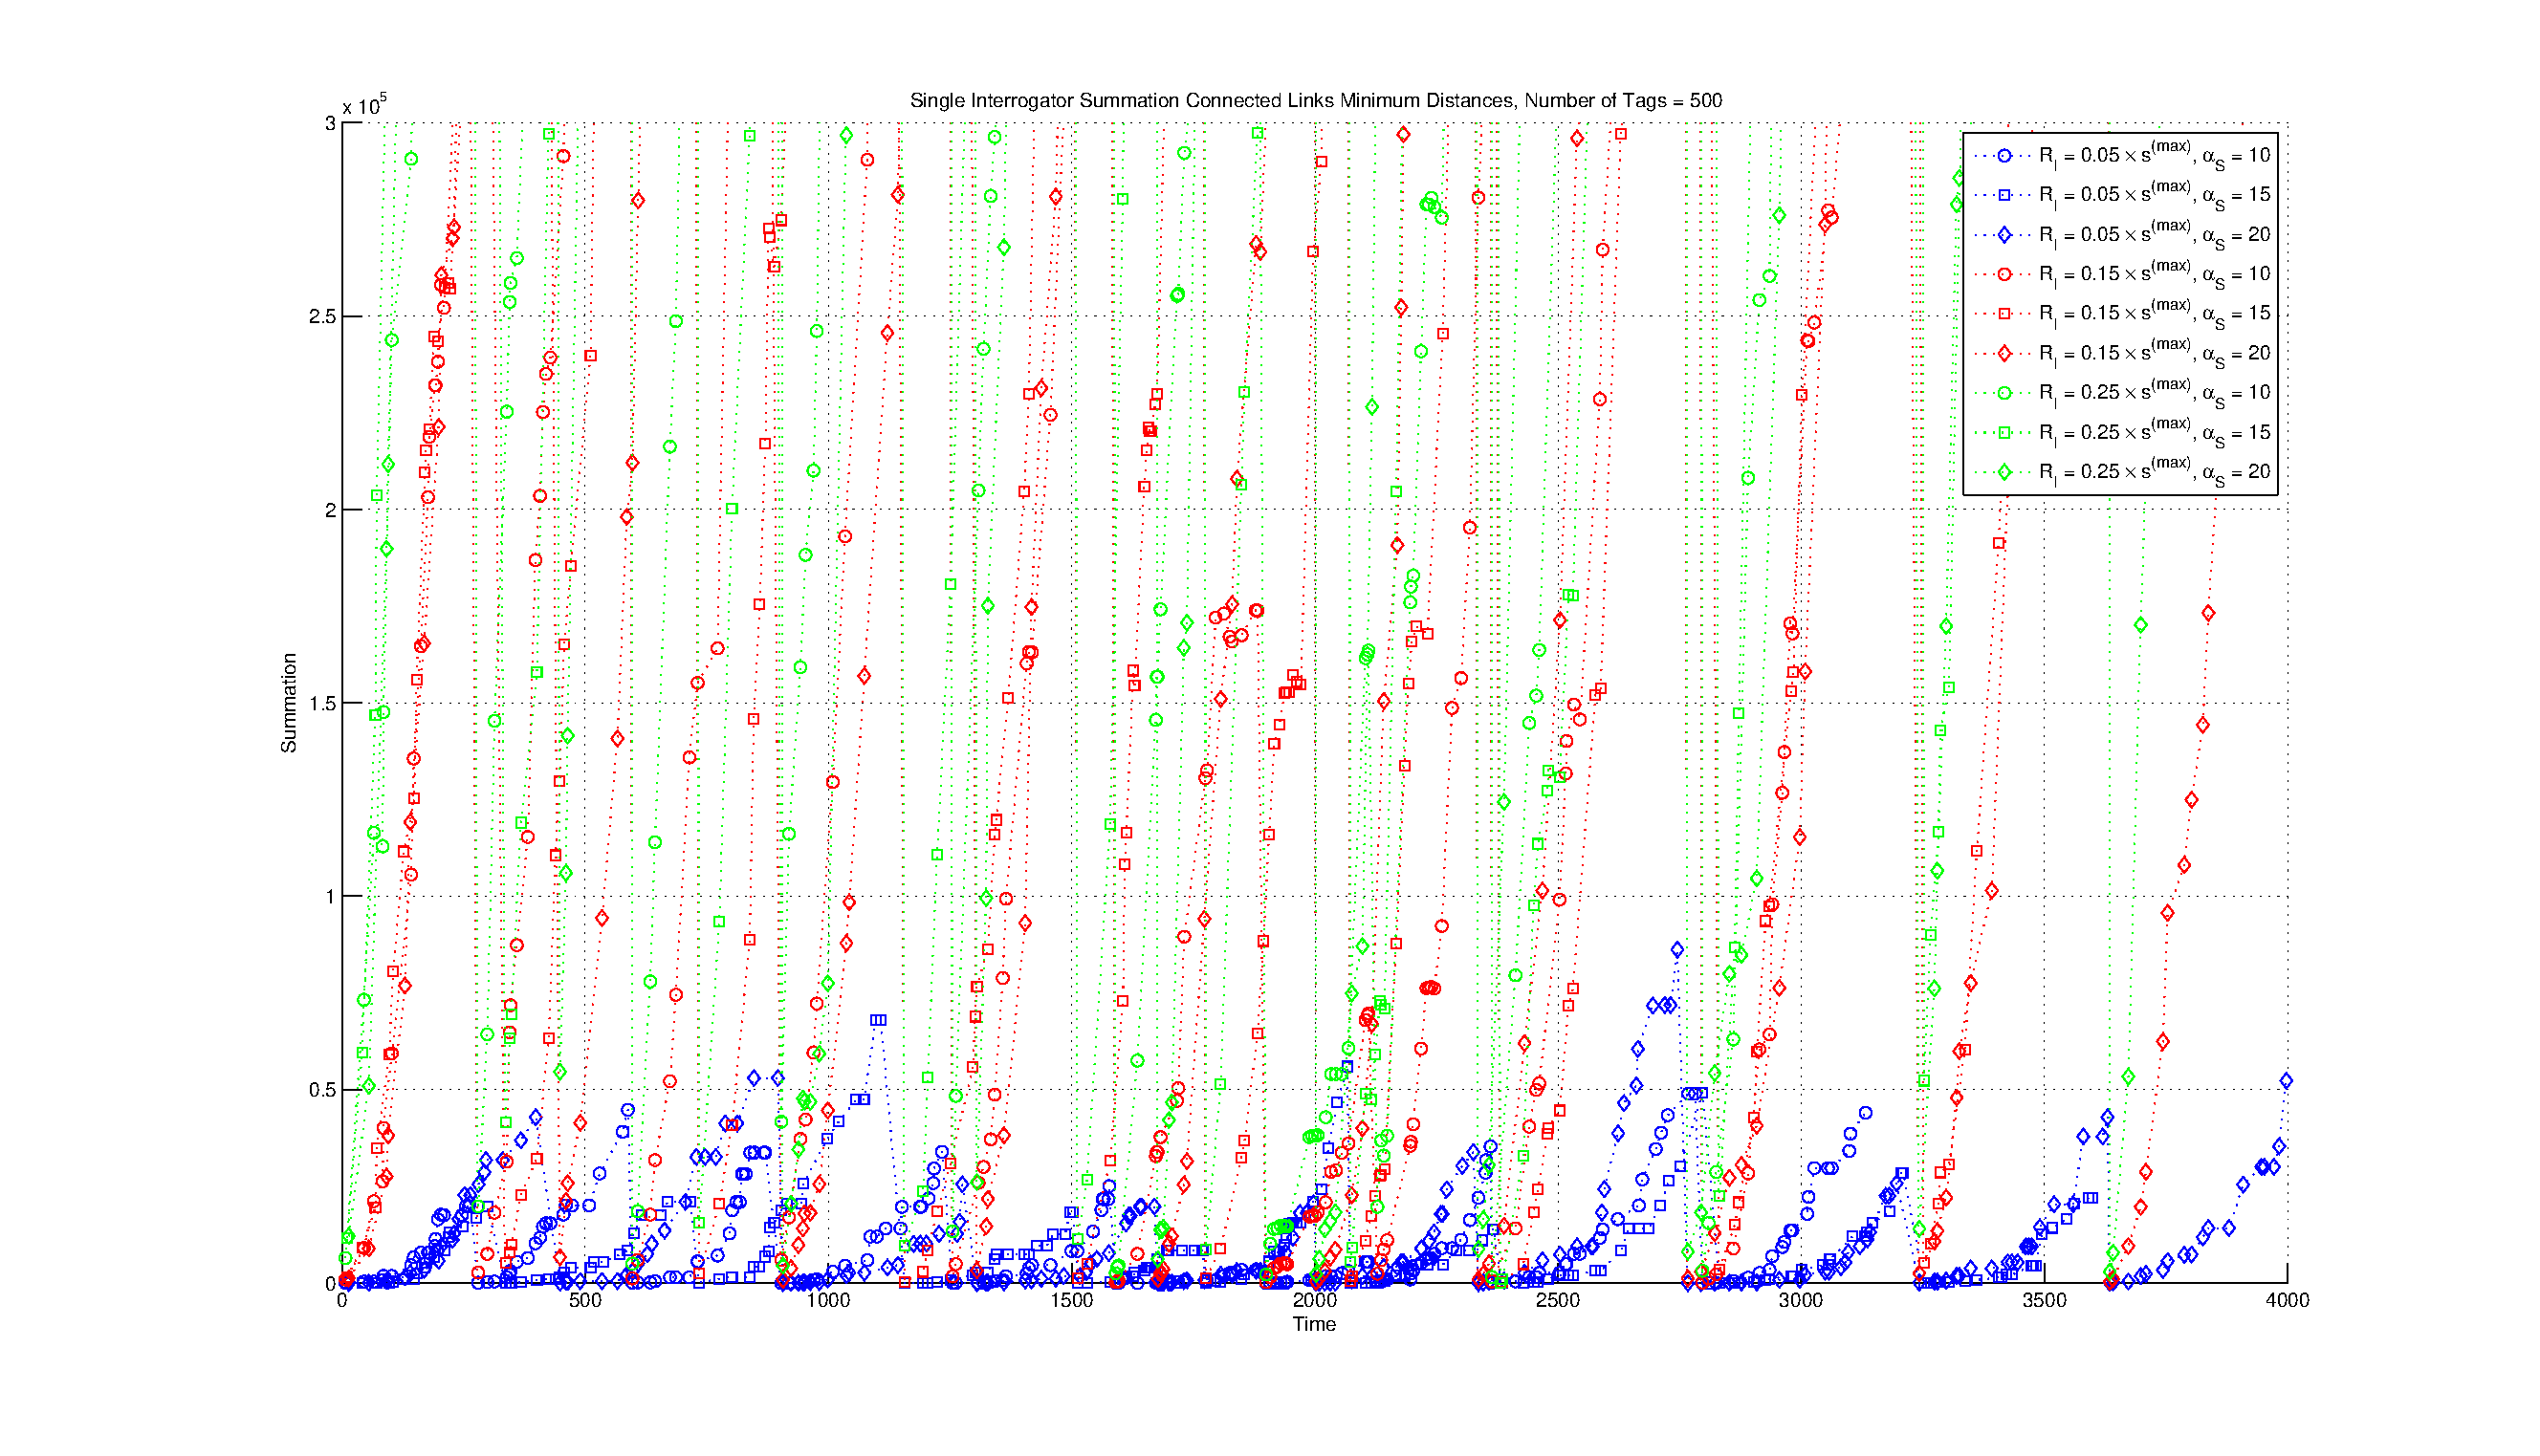
\includegraphics[width=5in, height=3.5in]{Chapter_4_Figures/sin_min_500tags_all.eps}
\caption{Single interrogator summation of connected links minimum distances. Number of tags = 500 and $R_I \in \{0.05, 0.15, 0.25\} \times s^{(max)}$.}
\label{Figure: sin_min_500tags_all.eps}
\end{figure}
\begin{figure}
\centering
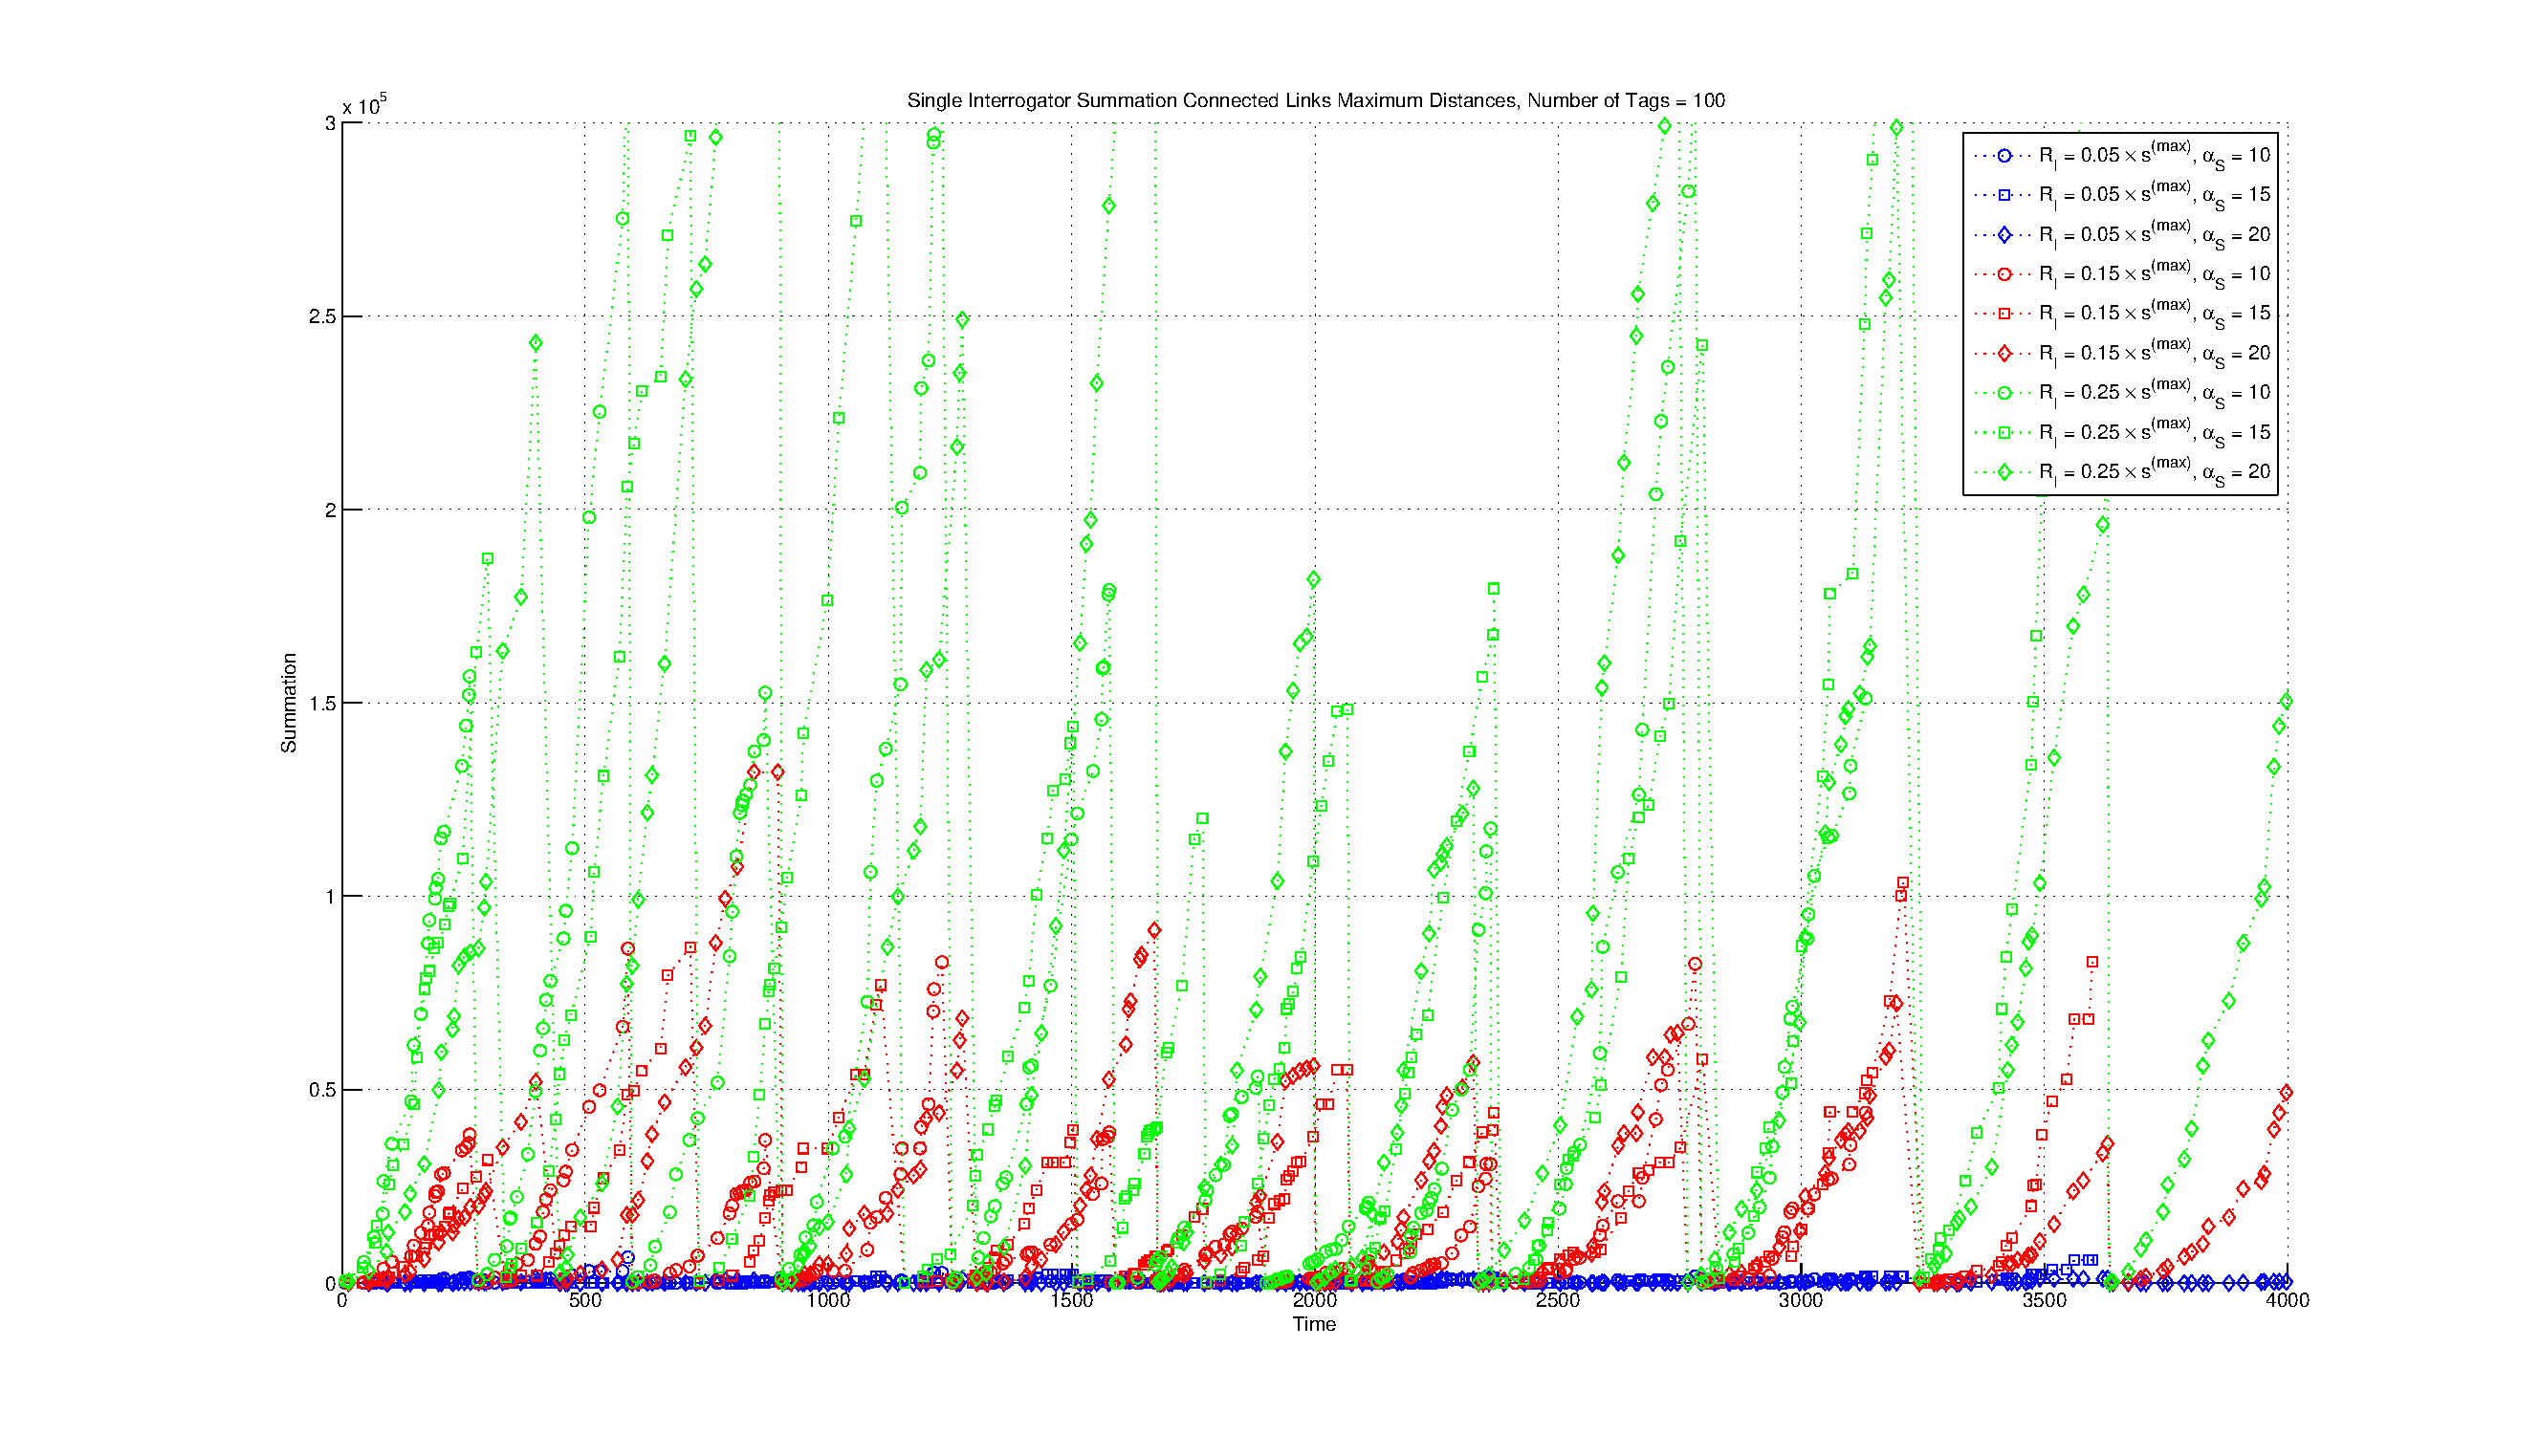
\includegraphics[width=5in, height=3.5in]{Chapter_4_Figures/sin_max_100tags_all.eps}
\caption{Single interrogator summation of connected links maximum distances. Number of tags = 100 and $R_I \in \{0.05, 0.15, 0.25\} \times s^{(max)}$.}
\label{Figure: sin_max_100tags_all.eps}
\end{figure}
\clearpage

\begin{figure}
\centering
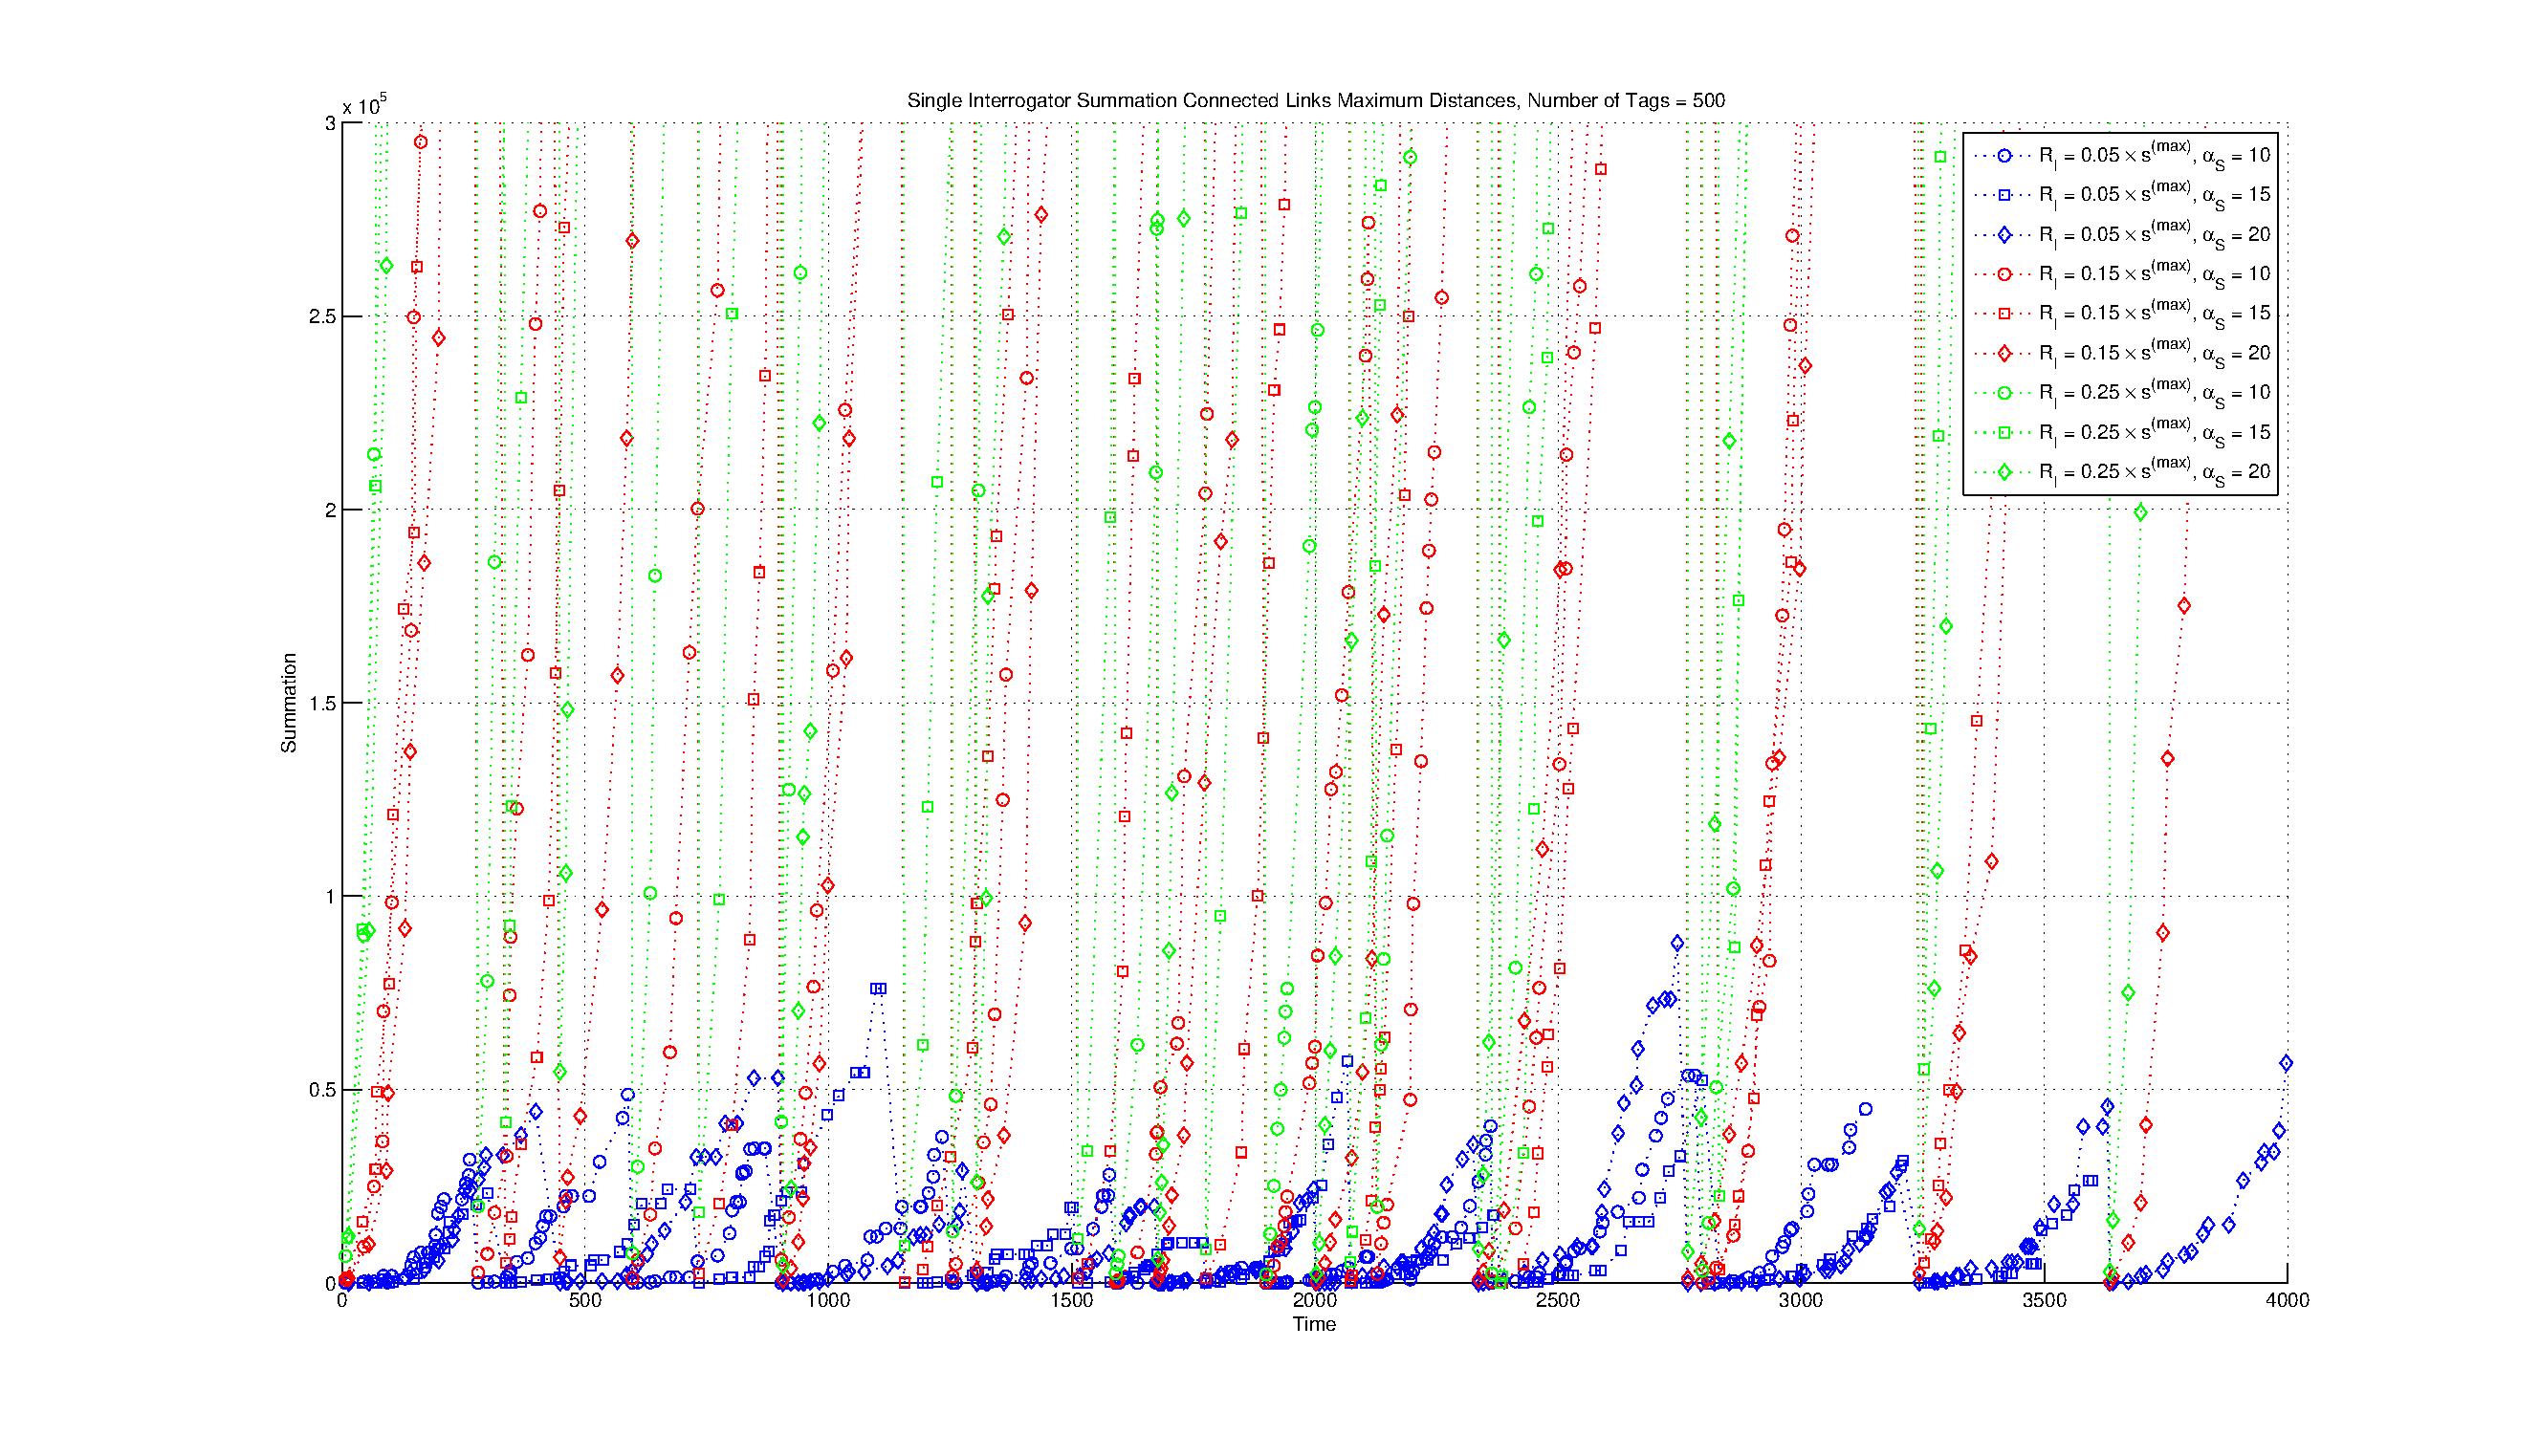
\includegraphics[width=5in, height=3.5in]{Chapter_4_Figures/sin_max_500tags_all.eps}
\caption{Single interrogator summation of connected links maximum distances. Number of tags = 500 and $R_I \in \{0.05, 0.15, 0.25\} \times s^{(max)}$.}
\label{Figure: sin_max_500tags_all.eps}
\end{figure}
\begin{figure}
\centering
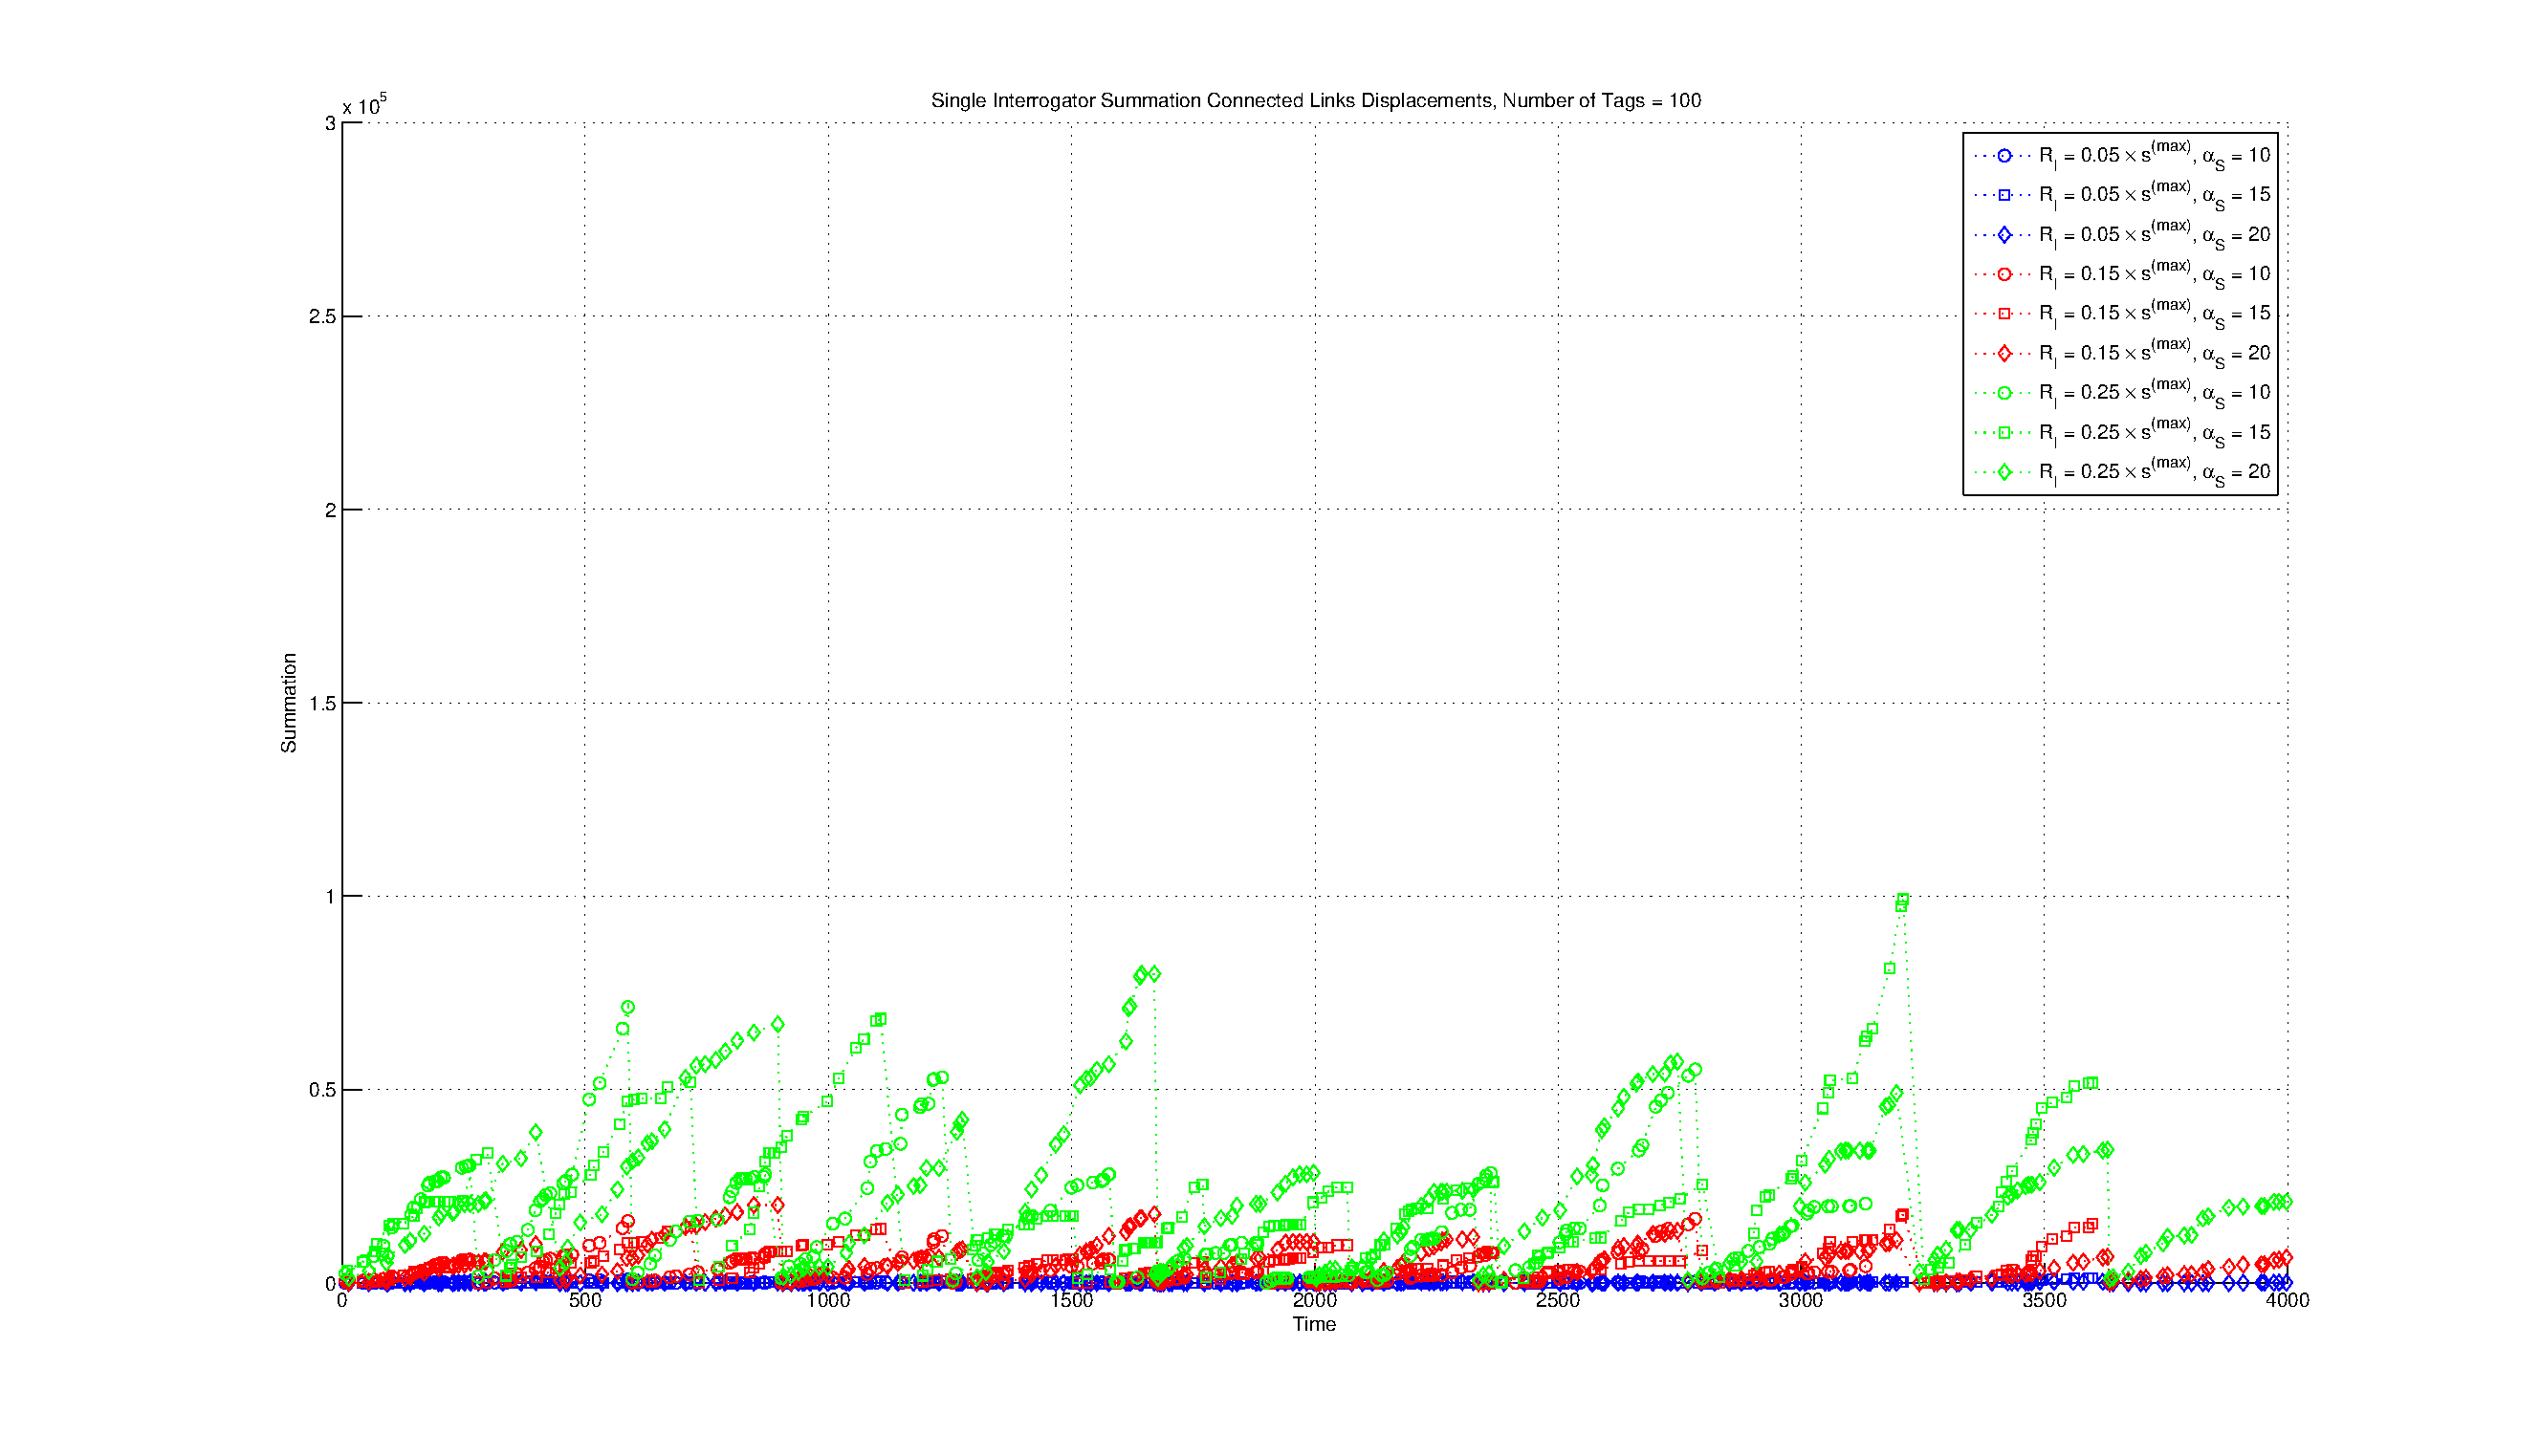
\includegraphics[width=5in, height=3.5in]{Chapter_4_Figures/sin_disp_100tags_all.eps}
\caption{Single interrogator summation of connected links displacements. Number of tags = 100 and $R_I \in \{0.05, 0.15, 0.25\} \times s^{(max)}$.}
\label{Figure: sin_disp_100tags_all.eps}
\end{figure}
\clearpage

\begin{figure}
\centering
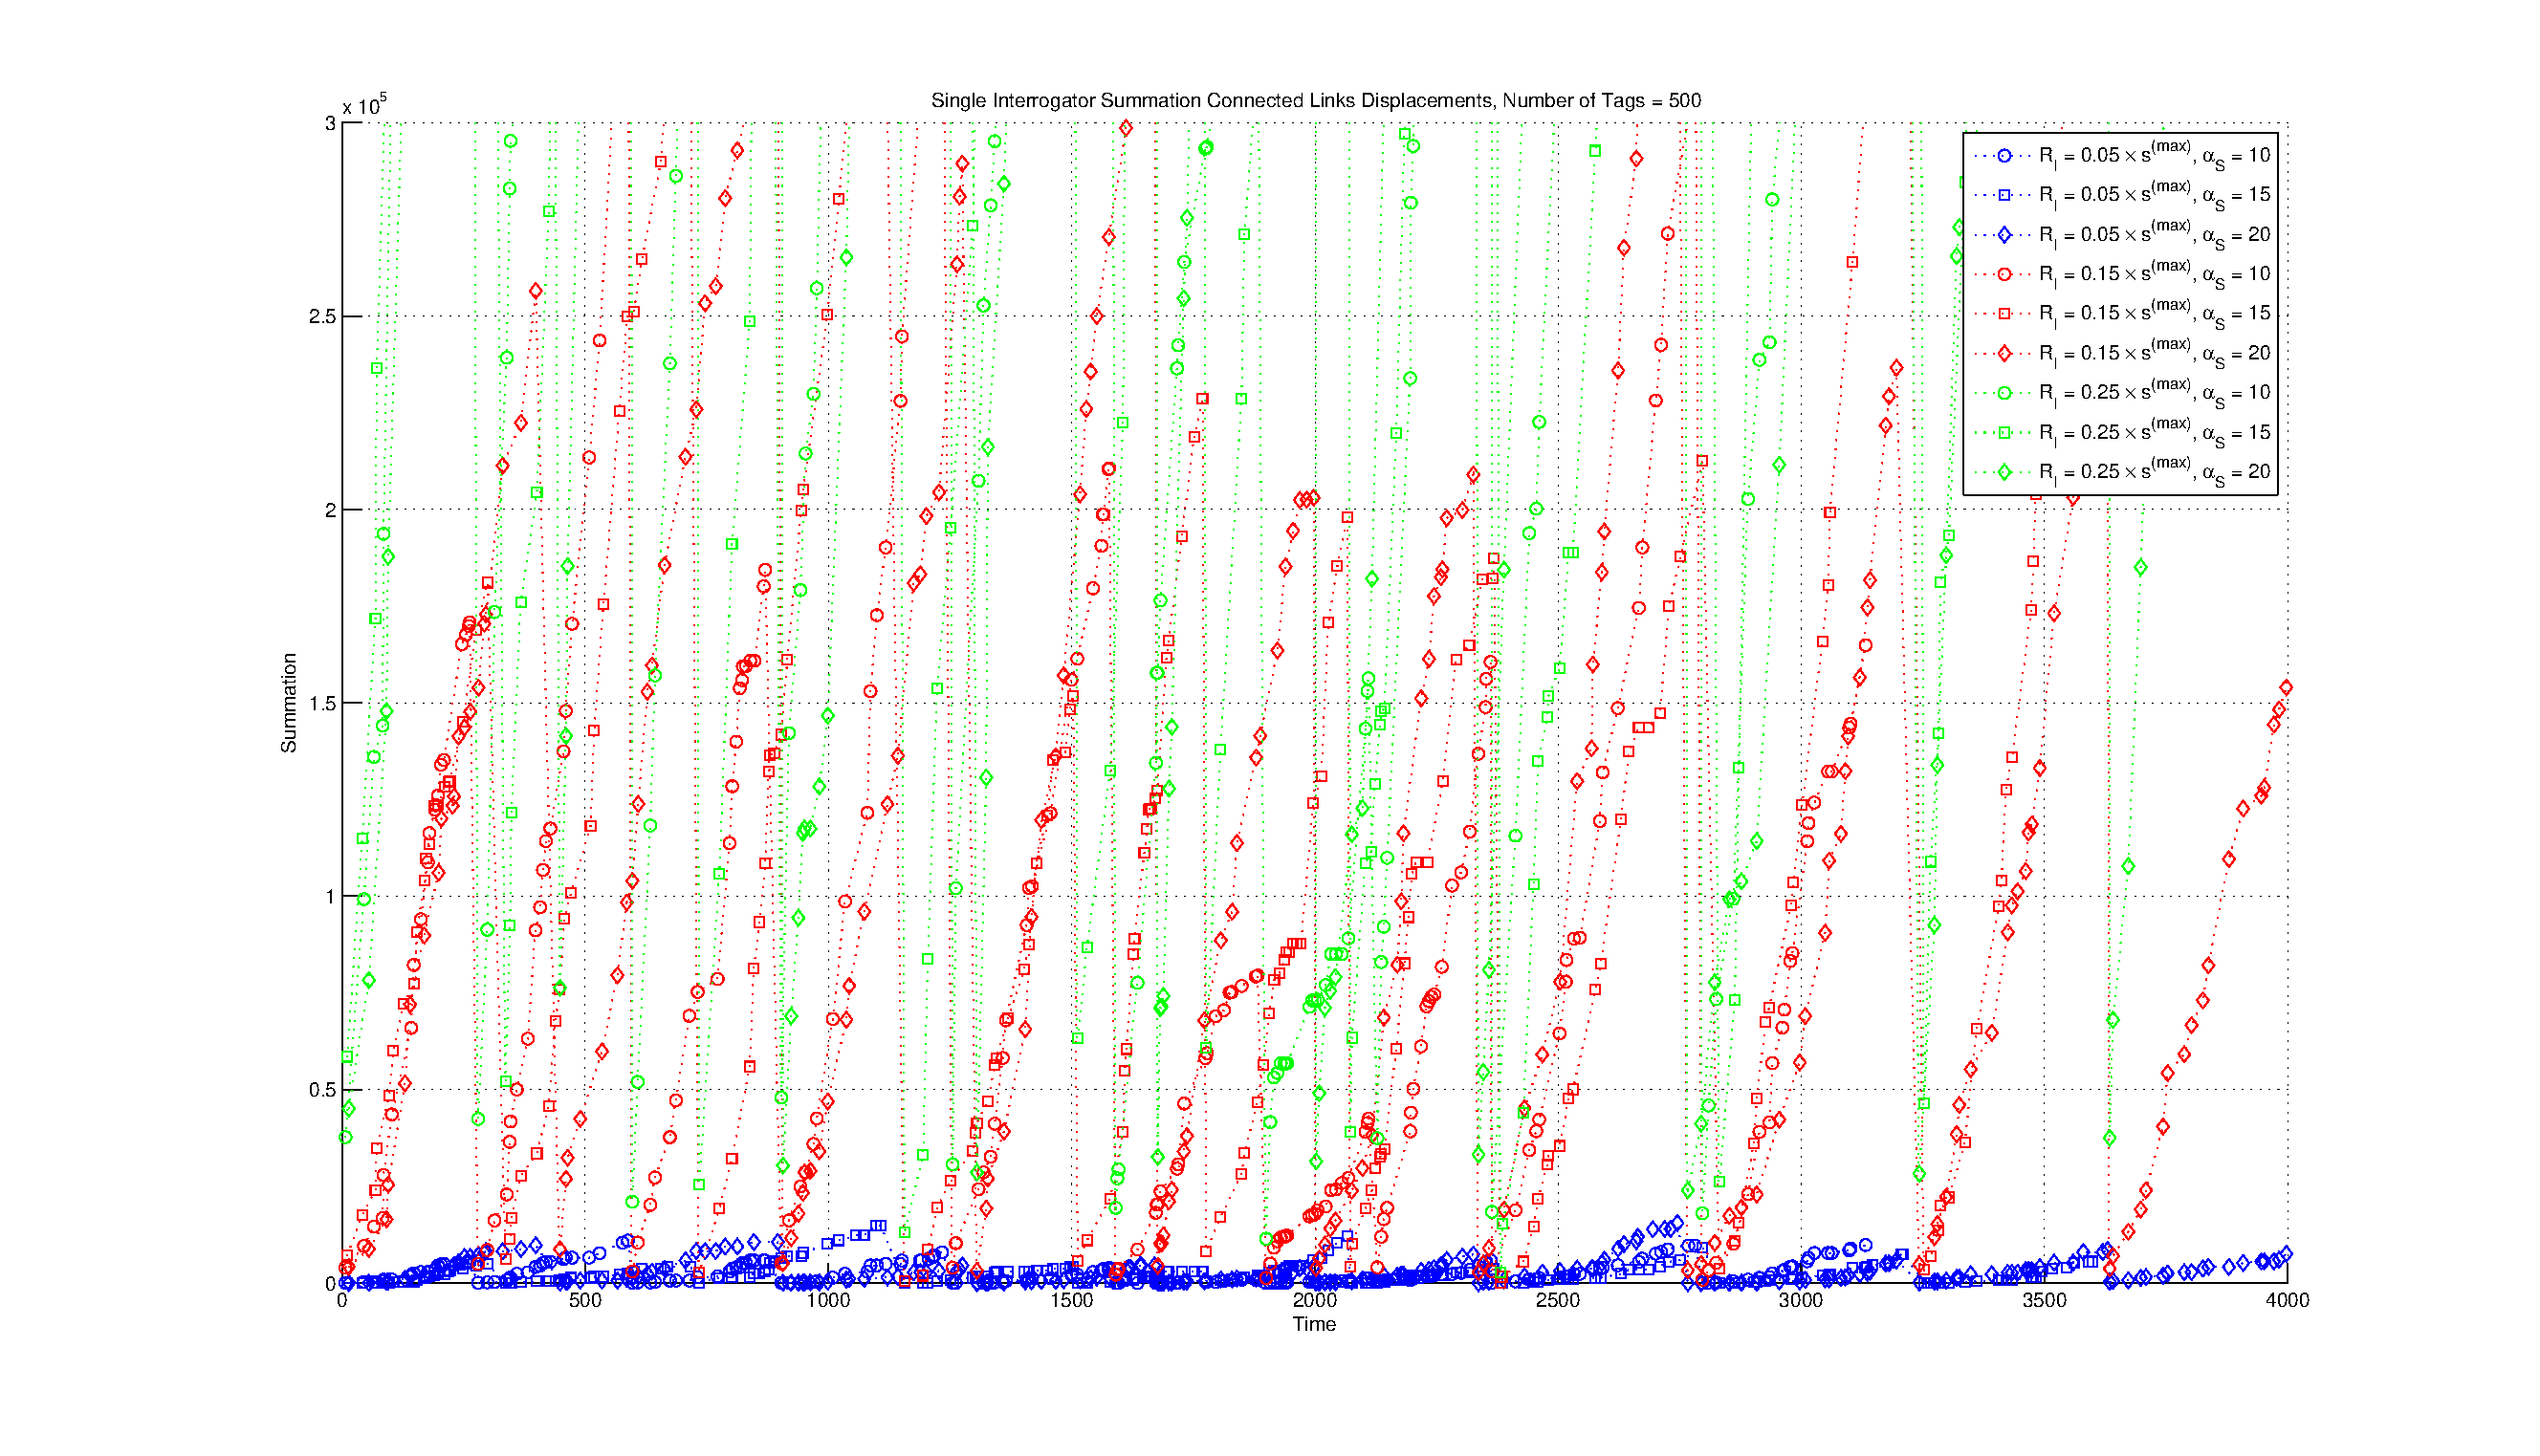
\includegraphics[width=5in, height=3.5in]{Chapter_4_Figures/sin_disp_500tags_all.eps}
\caption{Single interrogator summation of connected links displacements. Number of tags = 500 and $R_I \in \{0.05, 0.15, 0.25\} \times s^{(max)}$.}
\label{Figure: sin_disp_500tags_all.eps}
\end{figure}
\begin{figure}
\centering
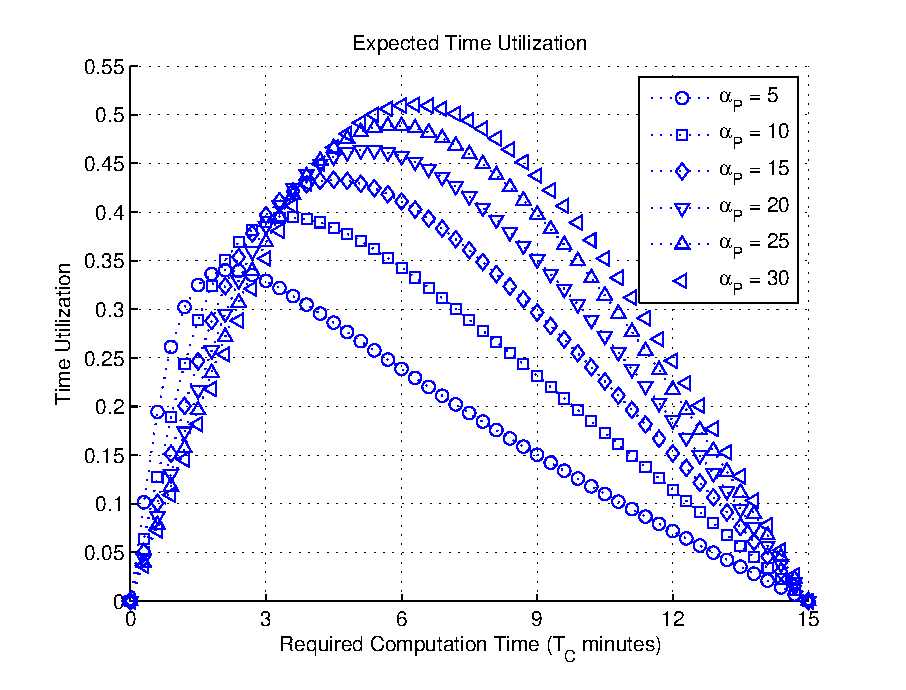
\includegraphics[width=5in]{Chapter_4_Figures/expect_time_util.eps}
\caption{Expected time utilization. $\alpha_P \in \{5, 10, 15, 20, 25, 30\}$.}
\label{Figure: expect_time_util.eps}
\end{figure}
\clearpage

\begin{figure}
\centering
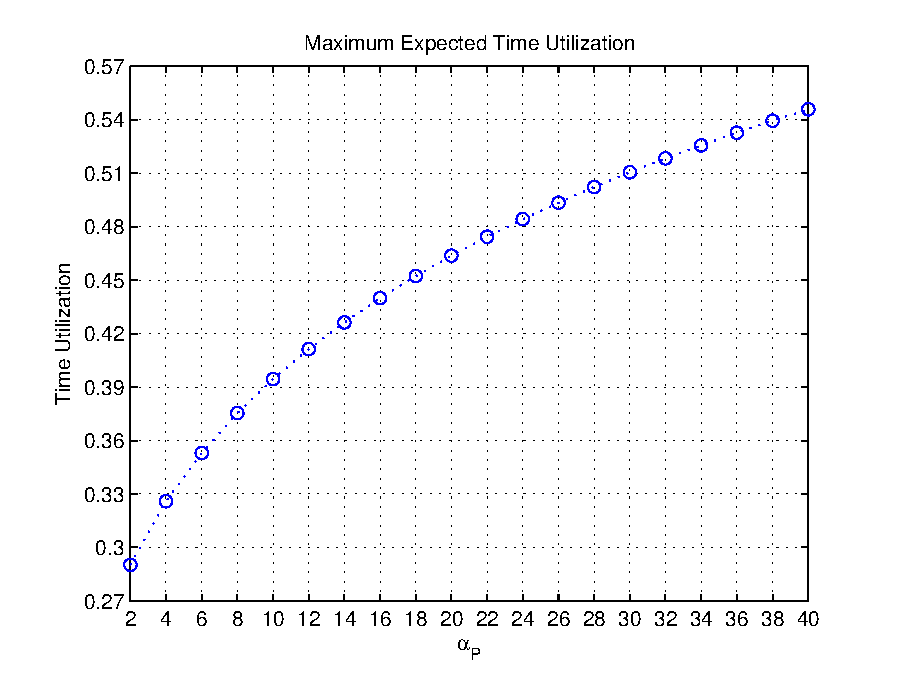
\includegraphics[width=5in]{Chapter_4_Figures/max_expect_time_util.eps}
\caption{Maximum expected time utilization.}
\label{Figure: max_expect_time_util.eps}
\end{figure}
\begin{figure}
\centering
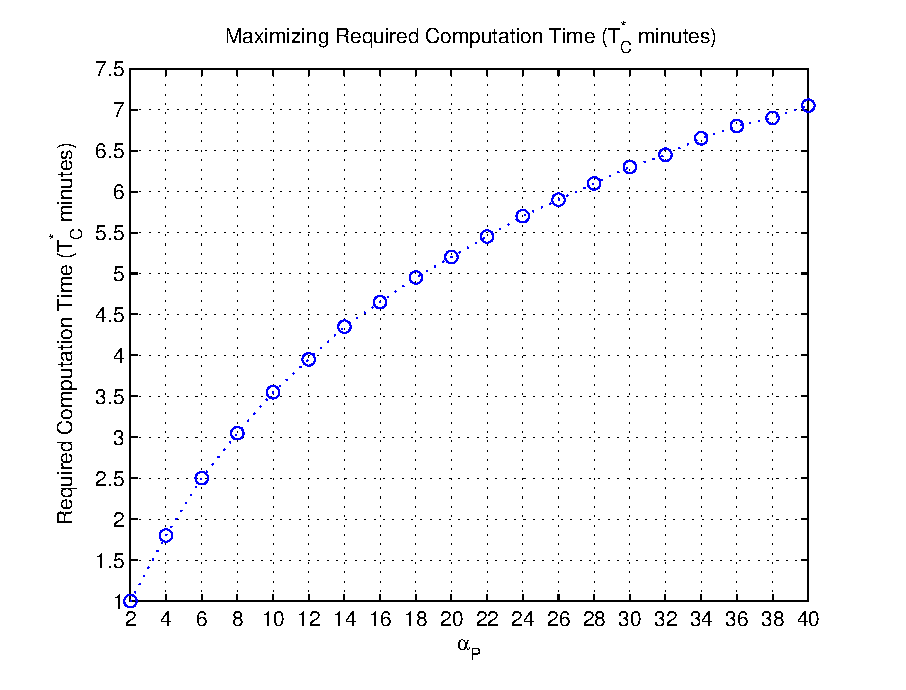
\includegraphics[width=5in]{Chapter_4_Figures/maximizing_compute_time.eps}
\caption{Maximizing required computation time.}
\label{Figure: maximizing_compute_time.eps}
\end{figure}
\clearpage

\begin{table}
\caption{Range of computing speeds (instructions$/$second).}
\label{Table: Range of computing speeds (instructions/second).}
\begin{center}
\begin{tabular}{|c|c|c|c|c|c|}
\hline
  & $\beta = 200$ & $\beta = 400$ & $\beta = 600$ & $\beta = 800$ & $\beta = 1000$ \\
\hline
$r = 32$ & $1632.65$ & $2191.78$ & $2474.23$ & $2644.63$ & $2758.62$ \\
\hline
$r = 64$ & $816.33$ & $1095.89$ & $1237.11$ & $1322.31$ & $1379.31$ \\
\hline
\end{tabular}
\end{center}
\end{table}